\def\bmode{2} % Mode 0 for presentation, mode 1 for a handout with notes, mode 2 for handout without notes
\if 0\bmode
\documentclass[usenames,dvipsnames,smaller]{beamer}
\else \if 1\bmode
\immediate\write18{pdflatex -jobname=\jobname-Handout-Notes\space\jobname}
\documentclass[usenames,dvipsnames,smaller,handout]{beamer}
\usepackage{handoutWithNotes}
\pgfpagesuselayout{2 on 1 with notes}[letterpaper, landscape, border shrink=4mm]
\else \if 2\bmode
\immediate\write18{pdflatex -jobname=\jobname-Handout\space\jobname}
\documentclass[usenames,dvipsnames,smaller,handout]{beamer}
\fi
\fi
\fi

% \documentclass[usenames,dvipsnames,smaller,handout]{beamer}
% \usepackage{handoutWithNotes}
% \pgfpagesuselayout{2 on 1 with notes}[letterpaper, landscape, border shrink=4mm]

% \usepackage[T1]{fontenc} 
% \usepackage{lmodern} 
%\usepackage{etex}
 %\newcommand{\num}{6{} }

% \usetheme[
%   outer/progressbar=foot,
%   outer/numbering=fraction,
%   block=fill,
%   inner/subsectionpage=progressbar
% ]{metropolis}
\usetheme{Madrid}
\useoutertheme[subsection=false]{miniframes} % Alternatively: miniframes, infolines, split
\useinnertheme{circles}
% %\useoutertheme{Frankfurt}
% \usecolortheme{beaver}
% %\useoutertheme{crane}
% %\useoutertheme{metropolis}
\usepackage[backend=biber,style=authoryear,maxcitenames=2,maxbibnames=99,safeinputenc,url=false, eprint=false]{biblatex}
%\addbibresource{bib/references.bib}
% \AtEveryCitekey{\iffootnote{{\tiny}\tiny}{\tiny}}

% %\usepackage{pgfpages}
% %\setbeameroption{hide notes} % Only slides
% %\setbeameroption{show only notes} % Only notes
% %\setbeameroption{hide notes} % Only notes
% %\setbeameroption{show notes on second screen=right} % Both

% % \usepackage[sfdefault]{Fira Sans}

% % \setsansfont[BoldFont={Fira Sans}]{Fira Sans Light}
% % \setmonofont{Fira Mono}

% %\usepackage{fira}
% %\setsansfont{Fira}
% %\setmonofont{Fira Mono}
% % To give a presentation with the Skim reader (http://skim-app.sourceforge.net) on OSX so
% % that you see the notes on your laptop and the slides on the projector, do the following:
% % 
% % 1. Generate just the presentation (hide notes) and save to slides.pdf
% % 2. Generate onlt the notes (show only nodes) and save to notes.pdf
% % 3. With Skim open both slides.pdf and notes.pdf
% % 4. Click on slides.pdf to bring it to front.
% % 5. In Skim, under "View -> Presentation Option -> Synhcronized Noted Document"
% %    select notes.pdf.
% % 6. Now as you move around in slides.pdf the notes.pdf file will follow you.
% % 7. Arrange windows so that notes.pdf is in full screen mode on your laptop
% %    and slides.pdf is in presentation mode on the projector.

% % Give a slight yellow tint to the notes page
% \setbeamertemplate{note page}{\pagecolor{yellow!5}\insertnote}\usepackage{palatino}

% %\usetheme{metropolis}
% %\usecolortheme{beaver}
 \usepackage{tipa}
% \usepackage{enumerate}
% \definecolor{darkcandyapplered}{HTML}{A40000}
% \definecolor{lightcandyapplered}{HTML}{e74c3c}

% %\setbeamercolor{title}{fg=darkcandyapplered}

% \definecolor{UBCblue}{rgb}{0.04706, 0.13725, 0.26667} % UBC Blue (primary)
% \definecolor{UBCgrey}{rgb}{0.3686, 0.5255, 0.6235} % UBC Grey (secondary)

% % \setbeamercolor{palette primary}{bg=darkcandyapplered,fg=white}
% % \setbeamercolor{palette secondary}{bg=darkcandyapplered,fg=white}
% % \setbeamercolor{palette tertiary}{bg=darkcandyapplered,fg=white}
% % \setbeamercolor{palette quaternary}{bg=darkcandyapplered,fg=white}
% % \setbeamercolor{structure}{fg=darkcandyapplered} % itemize, enumerate, etc
% % \setbeamercolor{section in toc}{fg=darkcandyapplered} % TOC sections
% % \setbeamercolor{frametitle}{fg=darkcandyapplered,bg=white} % TOC sections
% % \setbeamercolor{title in head/foot}{bg=white,fg=white} % TOC sections
% % \setbeamercolor{button}{fg=darkcandyapplered} % TOC sections

% % % Override palette coloring with secondary
% % \setbeamercolor{subsection in head/foot}{bg=lightcandyapplered,fg=white}

%\usecolortheme{crane}
% \makeatletter
% \setbeamertemplate{headline}{%
%   \begin{beamercolorbox}[colsep=1.5pt]{upper separation line head}
%   \end{beamercolorbox}
%   \begin{beamercolorbox}{section in head/foot}
%     \vskip1pt\insertsectionnavigationhorizontal{\paperwidth}{}{}\vskip1pt
%   \end{beamercolorbox}%
%   \ifbeamer@theme@subsection%
%     \begin{beamercolorbox}[colsep=1.5pt]{middle separation line head}
%     \end{beamercolorbox}
%     \begin{beamercolorbox}[ht=2.5ex,dp=1.125ex,%
%       leftskip=.3cm,rightskip=.3cm plus1fil]{subsection in head/foot}
%       \usebeamerfont{subsection in head/foot}\insertsubsectionhead
%     \end{beamercolorbox}%
%   \fi%
%   \begin{beamercolorbox}[colsep=1.5pt]{lower separation line head}
%   \end{beamercolorbox}
% }
% \makeatother

% Reduce size of frame box
\setbeamertemplate{frametitle}{%
    \nointerlineskip%
    \begin{beamercolorbox}[wd=\paperwidth,ht=2.0ex,dp=0.6ex]{frametitle}
        \hspace*{1ex}\insertframetitle%
    \end{beamercolorbox}%
}


%\setbeamercolor{frametitle}{bg=darkcandyapplered!80!black!90!white}
%\setbeamertemplate{frametitle}{\bf\insertframetitle}

%\setbeamercolor{footnote mark}{fg=darkcandyapplered}
%\setbeamercolor{footnote}{fg=darkcandyapplered!70}
%\Raggedbottom
%\setbeamerfont{page number in head/foot}{size=\tiny}
%\usepackage[tracking]{microtype}


% %\usepackage[sc,osf]{mathpazo}   % With old-style figures and real smallcaps.
% %\linespread{1.025}              % Palatino leads a little more leading

% % Euler for math and numbers
% %\usepackage[euler-digits,small]{eulervm}
% %\AtBeginDocument{\renewcommand{\hbar}{\hslash}}
\usepackage{graphicx,multirow,booktabs}


% %\mode<presentation> { \setbeamercovered{transparent} }

\setbeamertemplate{navigation symbols}{}
\makeatletter
\def\beamerorig@set@color{%
  \pdfliteral{\current@color}%
  \aftergroup\reset@color
}
\def\beamerorig@reset@color{\pdfliteral{\current@color}}
\makeatother


% %=== GRAPHICS PATH ===========
\graphicspath{{./images/}}
% % Marginpar width
% %Marginpar width
% %\setlength{\marginparsep}{.02in}


% %% Captions
% % \usepackage{caption}
% % \captionsetup{
% %   labelsep=quad,
% %   justification=raggedright,
% %   labelfont=sc
% % }

% \setbeamerfont{caption}{size=\footnotesize}
% \setbeamercolor{caption name}{fg=darkcandyapplered}

% %AMS-TeX packages

\usepackage{amssymb,amsmath,amsthm,mathtools} 
\usepackage{bm, mathrsfs}
% \usepackage{color}

% %https://tex.stackexchange.com/a/31370/2269
% \usepackage{mathtools,cancel}

% \renewcommand{\CancelColor}{\color{red}} %change cancel color to red

% \makeatletter
% \let\my@cancelto\cancelto %copy over the original cancelto command
% \newcommand<>{\cancelto}[2]{\alt#3{\my@cancelto{#1}{#2}}{\mathrlap{#2}\phantom{\my@cancelto{#1}{#2}}}}
% % redefine the cancelto command, using \phantom to assure that the
% % result doesn't wiggle up and down with and without the arrow
% \makeatother


% %\usepackage{comment}
% %\usepackage{hyperref,enumerate}
% \usepackage{minitoc,array}

% \definecolor{slblue}{rgb}{0,.3,.62}
% % \hypersetup{
% %     colorlinks,%
% %     citecolor=blue,%
% %     filecolor=blue,%
% %     linkcolor=blue,
% %     urlcolor=slblue
% % }

% \usepackage{epstopdf}
% \epstopdfDeclareGraphicsRule{.gif}{png}{.png}{convert gif:#1 png:\OutputFile}
% \AppendGraphicsExtensions{.gif}

% %\usepackage{listings}

% %%% TIKZ
% \usepackage{forest}
\usepackage{tikz}
\usepackage{pgfplots}
\usepackage{pgfplotstable}
%\usepackage{pgfgantt}
\pgfplotsset{compat=newest}

\usetikzlibrary{fit,arrows,shapes,positioning,shapes.geometric}
\usetikzlibrary{decorations.markings}
\usetikzlibrary{shadows,automata}
\usetikzlibrary{patterns}
\usetikzlibrary{trees,mindmap,backgrounds}
%\usetikzlibrary{circuits.ee.IEC}
\usetikzlibrary{decorations.text}
% % For Sagnac Picture
% \usetikzlibrary{%
%     decorations.pathreplacing,%
%     decorations.pathmorphing%
% }
% \tikzset{no shadows/.style={general shadow/.style=}}
% %
% %\usepackage{paralist}

% \tikzset{
%   font=\Large\sffamily\bfseries,
%   red arrow/.style={
%     midway,red,sloped,fill, minimum height=3cm, single arrow, single arrow head extend=.5cm, single arrow head indent=.25cm,xscale=0.3,yscale=0.15,
%     allow upside down
%   },
%   black arrow/.style 2 args={-stealth, shorten >=#1, shorten <=#2},
%   black arrow/.default={1mm}{1mm},
%   tree box/.style={draw, rounded corners, inner sep=1em},
%   node box/.style={white, draw=black, text=black, rectangle, rounded corners},
% }

% %%% FORMAT PYTHON CODE
% %\usepackage{listings}
% % Default fixed font does not support bold face
% \DeclareFixedFont{\ttb}{T1}{txtt}{bx}{n}{8} % for bold
% \DeclareFixedFont{\ttm}{T1}{txtt}{m}{n}{8}  % for normal

% % Custom colors
% \definecolor{deepblue}{rgb}{0,0,0.5}
% \definecolor{deepred}{rgb}{0.6,0,0}
% \definecolor{deepgreen}{rgb}{0,0.5,0}

% %\usepackage{animate}

% % Python style for highlighting
% % \newcommand\pythonstyle{\lstset{
% % language=Python,
% % basicstyle=\footnotesize\ttm,
% % otherkeywords={self},             % Add keywords here
% % keywordstyle=\footnotesize\ttb\color{deepblue},
% % emph={MyClass,__init__},          % Custom highlighting
% % emphstyle=\footnotesize\ttb\color{deepred},    % Custom highlighting style
% % stringstyle=\color{deepgreen},
% % frame=tb,                         % Any extra options here
%     % showstringspaces=false            % 
% % }}

% % % Python environment
% % \lstnewenvironment{python}[1][]
% % {
% % \pythonstyle
% % \lstset{#1}
% % }
% % {}

% % % Python for external files
% % \newcommand\pythonexternal[2][]{{
% % \pythonstyle
% % \lstinputlisting[#1]{#2}}}

% % Python for inline
% % 
% % \newcommand\pythoninline[1]{{\pythonstyle\lstinline!#1!}}

% %\usepackage{algorithm2e}

\newcommand{\eps}{\epsilon}
\newcommand{\bX}{\mb X}
\newcommand{\by}{\mb y}
\newcommand{\bbe}{\bm\beta}
\newcommand{\beps}{\bm\epsilon}
\newcommand{\bY}{\mb Y}

\newcommand{\osn}{\oldstylenums}
\newcommand{\dg}{^{\circ}}
\newcommand{\lt}{\left}
\newcommand{\rt}{\right}
\newcommand{\pt}{\phantom}
\newcommand{\tf}{\therefore}
\newcommand{\?}{\stackrel{?}{=}}
\newcommand{\fr}{\frac}
\newcommand{\dfr}{\dfrac}
\newcommand{\ul}{\underline}
\newcommand{\tn}{\tabularnewline}
\newcommand{\nl}{\newline}
\newcommand\relph[1]{\mathrel{\phantom{#1}}}
\newcommand{\cm}{\checkmark}
\newcommand{\ol}{\overline}
\newcommand{\rd}{\color{red}}
\newcommand{\bl}{\color{blue}}
\newcommand{\pl}{\color{purple}}
\newcommand{\og}{\color{orange!90!black}}
\newcommand{\gr}{\color{green!40!black}}
\newcommand{\dca}{\color{darkcandyapplered}}
\newcommand{\nin}{\noindent}
\newcommand*\circled[1]{\tikz[baseline=(char.base)]{
            \node[shape=circle,draw,thick,inner sep=1pt] (char) {\small #1};}}

\newcommand{\bc}{\begin{compactenum}[\quad--]}
\newcommand{\ec}{\end{compactenum}}

\newcommand{\p}{\partial}
\newcommand{\pd}[2]{\frac{\partial{#1}}{\partial{#2}}}
\newcommand{\dpd}[2]{\dfrac{\partial{#1}}{\partial{#2}}}
\newcommand{\pdd}[2]{\frac{\partial^2{#1}}{\partial{#2}^2}}
\newcommand{\pde}[3]{\frac{\partial^2{#1}}{\partial{#2}\partial{#3}}}
\newcommand{\nmfr}[3]{\Phi\left(\frac{{#1} - {#2}}{#3}\right)}
\newcommand{\Err}{\text{Err}}
\newcommand{\err}{\text{err}}

%\DeclarePairedDelimiter\ceil{\lceil}{\rceil}
%\DeclarePairedDelimiter\floor{\lfloor}{\rfloor}

%%%% GREEK LETTER SHORTCUTS %%%%%
\newcommand{\la}{\lambda}
\renewcommand{\th}{\theta}
\newcommand{\al}{\alpha}
\newcommand{\G}{\Gamma}
\newcommand{\si}{\sigma}
\newcommand{\Si}{\Sigma}


\pgfmathdeclarefunction{poiss}{1}{%
  \pgfmathparse{(#1^x)*exp(-#1)/(x!)}%
  }

\pgfmathdeclarefunction{gauss}{2}{%
  \pgfmathparse{1/(#2*sqrt(2*pi))*exp(-((x-#1)^2)/(2*#2^2))}%
}

\pgfmathdeclarefunction{expo}{2}{%
  \pgfmathparse{#1*exp(-#1*#2)}%
}

\pgfmathdeclarefunction{expocdf}{2}{%
  \pgfmathparse{1 -exp(-#1*#2)}%
}


% \usepackage{pst-plot}

% \usepackage{pstricks-add}
% \usepackage{auto-pst-pdf}   

% \psset{unit = 3}

% \def\target(#1,#2){%
%  {\psset{fillstyle = solid}
%   \rput(#1,#2){%
%     \pscircle[fillcolor = white](0.7,0.7){0.7}
%     \pscircle[fillcolor = blue!60](0.7,0.7){0.5}
%     \pscircle[fillcolor = white](0.7,0.7){0.3}
%     \pscircle[fillcolor = red!80](0.7,0.7){0.1}}}}
% \def\dots[#1](#2,#3){%
%     \psRandom[
%       dotsize = 2pt,
%       randomPoints = 25
%     ](!#2 #1 0.04 sub sub #3 #1 0.04 sub sub)%
%      (!#2 #1 0.04 sub add #3 #1 0.04 sub add)%
%      {\pscircle[linestyle = none](#2,#3){#1}}}

%%%%%%%%%%%%%%%%%%%%%%%%%%%%%%%%%%%%%%%%%%%%%%%%%%%
%%%%%%%%%%%%%%%%%%%%%%%%%%%%%%%%%%%%%%%%%%%%%%%%%%%
\title[CEE 616: Foundations: Probability]{ {\normalsize CEE 616:  Probabilistic Machine Learning}
  \\ Lecture 1a: Foundations: Probability}
\date[Sep 2, 2025]{\footnotesize Feb 8, 2023}
\author{{\bf Jimi Oke}}
\institute[UMass Amherst]{
%\titlegraphic{\hfill
  \begin{tikzpicture}[baseline=(current bounding box.center)]
    \node[anchor=base] at (-7,0) (its) {
\includegraphics[scale=.3]{UMassEngineering_vert}} ;
  \end{tikzpicture}
  % \hfill\includegraphics[height=1.5cm]{logo}
}

%https://tex.stackexchange.com/questions/55806/mindmap-tikzpicture-in-beamer-reveal-step-by-step
  \tikzset{
    invisible/.style={opacity=0},
    visible on/.style={alt={#1{}{invisible}}},
    alt/.code args={<#1>#2#3}{%
      \alt<#1>{\pgfkeysalso{#2}}{\pgfkeysalso{#3}} % \pgfkeysalso doesn't change the path
    },
  }


% https://tex.stackexchange.com/questions/446468/labels-with-arrows-for-an-equation
% https://tex.stackexchange.com/a/402466/121799
\newcommand{\tikzmark}[3][]{
\ifmmode
\tikz[remember picture,baseline=(#2.base)] \node [inner sep=0pt,#1](#2) {$#3$};
\else
\tikz[remember picture,baseline=(#2.base)] \node [inner sep=0pt,#1](#2) {#3};
\fi
}

% \lstset{language=matlab,
%                 basicstyle=\scriptsize\ttfamily,
%                 keywordstyle=\color{blue}\ttfamily,
%                 stringstyle=\color{blue}\ttfamily,
%                 commentstyle=\color{gray}\ttfamily,
%                 morecomment=[l][\color{gray}]{\#}
%               }


              
\begin{document}

\maketitle





% \section{Syllabus}

% \begin{frame}
%   \frametitle{General information}
%   \pause
%   Syllabus available on Moodle.
  
% \end{frame}

% \begin{frame}
%   \frametitle{Course objectives}
%   \begin{itemize}[<+->]
% \item Understand the importance of big data and machine learning in engineering
% \item Create and train models for various problem structures and applications
% \item Understand the theory behind fundamental algorithms and apply them
% \end{itemize}

% \end{frame}

% \begin{frame}
%   \frametitle{Assessments}

%   \begin{enumerate}[<+->]
%   \item Problem Sets: 5 $\times$ 10\% $=$ 50\%
%   \item Midterm Exam 1: 15\%
%   \item Midterm Exam 2: 15\% 
%   \item Project: 20\%
%   \end{enumerate}
% \end{frame}

% \begin{frame}
%   \frametitle{Problem Sets}
%   \pause

%   \begin{itemize}[<+->]
%   \item 4 problem sets assigned biweekly on Fridays
%   \item Collaboration is encouraged (state who you worked with on your submission)
%   \item Submission via Moodle (PDF along with supporting scripts; or
%     Jupyter Notebook)
%   \item Late homework: 25\% penalty (and no later than the Monday after due date) 
%   \end{itemize}
% \end{frame}

% \begin{frame}
%   \frametitle{Term project}\pause

%   \begin{itemize}[<+->]
%   \item Opportunity to go deep and apply a combination of topics to area of choice
%   \item Proposals due on April 8
%   \item Individual or pairs allowed (include in proposal)
%   \item I will also provide  datasets and ideas as needed
%   \item Projects will be presented May 4 (reports due that week)
%   \end{itemize}
% \end{frame}


% \begin{frame}
%   \frametitle{Documentation}
  
%   \begin{block}{Readings}\pause
%     \begin{itemize}[<+->]
% \item   Hastie, T., Tibshirani, R., \& Friedman, J. (2017). \textit{The Elements of Statistical Learning: Data Mining, Inference and Prediction}. Springer, New York, NY. Second Edition. (This text, among other resources, is also freely available from the authors at \url{https://web.stanford.edu/~hastie/ElemStatLearn/}. Abbreviated as ``ESL'' in the schedule and lecture notes.)

% \item  James, G., Witten, D., Hastie, T., \& Tibshirani, R. (2017). \textit{An Introduction to Statistical Learning with Applications in R}. Springer, New York. (The text, among other resources is freely available from the author at \url{http://faculty.marshall.usc.edu/gareth-james/ISL/}, although you may prefer to buy a hard copy. Abbreviated as ``ISLR'' in the schedule  and lecture notes.)

% \item Goulet, J.-A.\ (2020) \texttt{Probabilistic Machine Learning for Civil Engineers}, The MIT Press. (This text is freely available at \url{http://profs.polymtl.ca/jagoulet/Site/Goulet_web_page_BOOK.html}. Abbreviated as ``PML'' in the schedule and lecture notes.)
% \end{itemize}
      
%     % \item Supplementary readings (book chapters, journal articles) will be provided on \href{https://moodle.umass.edu/course/view.php?id=64661}
%     %   {
\includegraphics[width=.1\textwidth]{moodle-logo}}
  
%   \end{block}
% \end{frame}

% \begin{frame}
%   \frametitle{Documentation (continued)}
%   \pause
  
%   \begin{block}{Handouts}
%     Lecture handouts will be available on Moodle before class
%   \end{block}

%   \pause

%   \begin{block}{Other}
%     \begin{itemize}
%     \item Programming examples used in class will be availabe on Moodle (either as scripts or as JupyterLab notebooks)
%     \item Review/practice questions may be provided before  exams
%     \end{itemize}
%   \end{block}
% \end{frame}


% \begin{frame}
%   \frametitle{Policies and values}
%   \begin{itemize}[<+->]
%   \item Intellectual curiosity and academic honesty
%   \item Active learning (class participation and engagement)
%   \item Inclusivity and equitability
%   \item Readings: best to do them before class
%   \item Attendance: you are expected to attend every class
%   \item Schedule may be adapted based on class progress/needs
%   \end{itemize}
% \end{frame}

% %\section{Overview of Topics}
% \begin{frame}
%   \frametitle{Modules}
%   \begin{enumerate}[<+->]
%   \item Introduction and Background
%   \item Regression and Classification
%   \item Model Assessment and Selection
%   \item Nonlinear Methods
%   \item Tree-Based Methods  
%   \item Support Vector Machines
%   \item Time Series Analysis
%   \item Unsupervised Learning    
%   \item Neural Networks
%   \end{enumerate}

%   \pause

  
% \end{frame}


\begin{frame}{Outline}
  \tableofcontents
\end{frame}

\section{Introduction}
% \begin{frame}
%   \frametitle{What is ``Big data''?}
%   \pause
  
%   \begin{center}
%     
\includegraphics[width=.5\textwidth]{big_data_cover}
%   \end{center}
%   \pause
  
%   \begin{block}{Definition}
%    \textit{Big Data} consists of extensive datasets---primarily in the characteristics of volume, variety, velocity,
%    and/or variability---that require a scalable architecture for efficient storage, manipulation, and analysis
%    (\href{https://bigdatawg.nist.gov/_uploadfiles/NIST.SP.1500-1.pdf}{NIST})
%  \end{block}
% \end{frame}


% % \begin{frame}
% %   \frametitle{Four V's of big data}\pause

% %   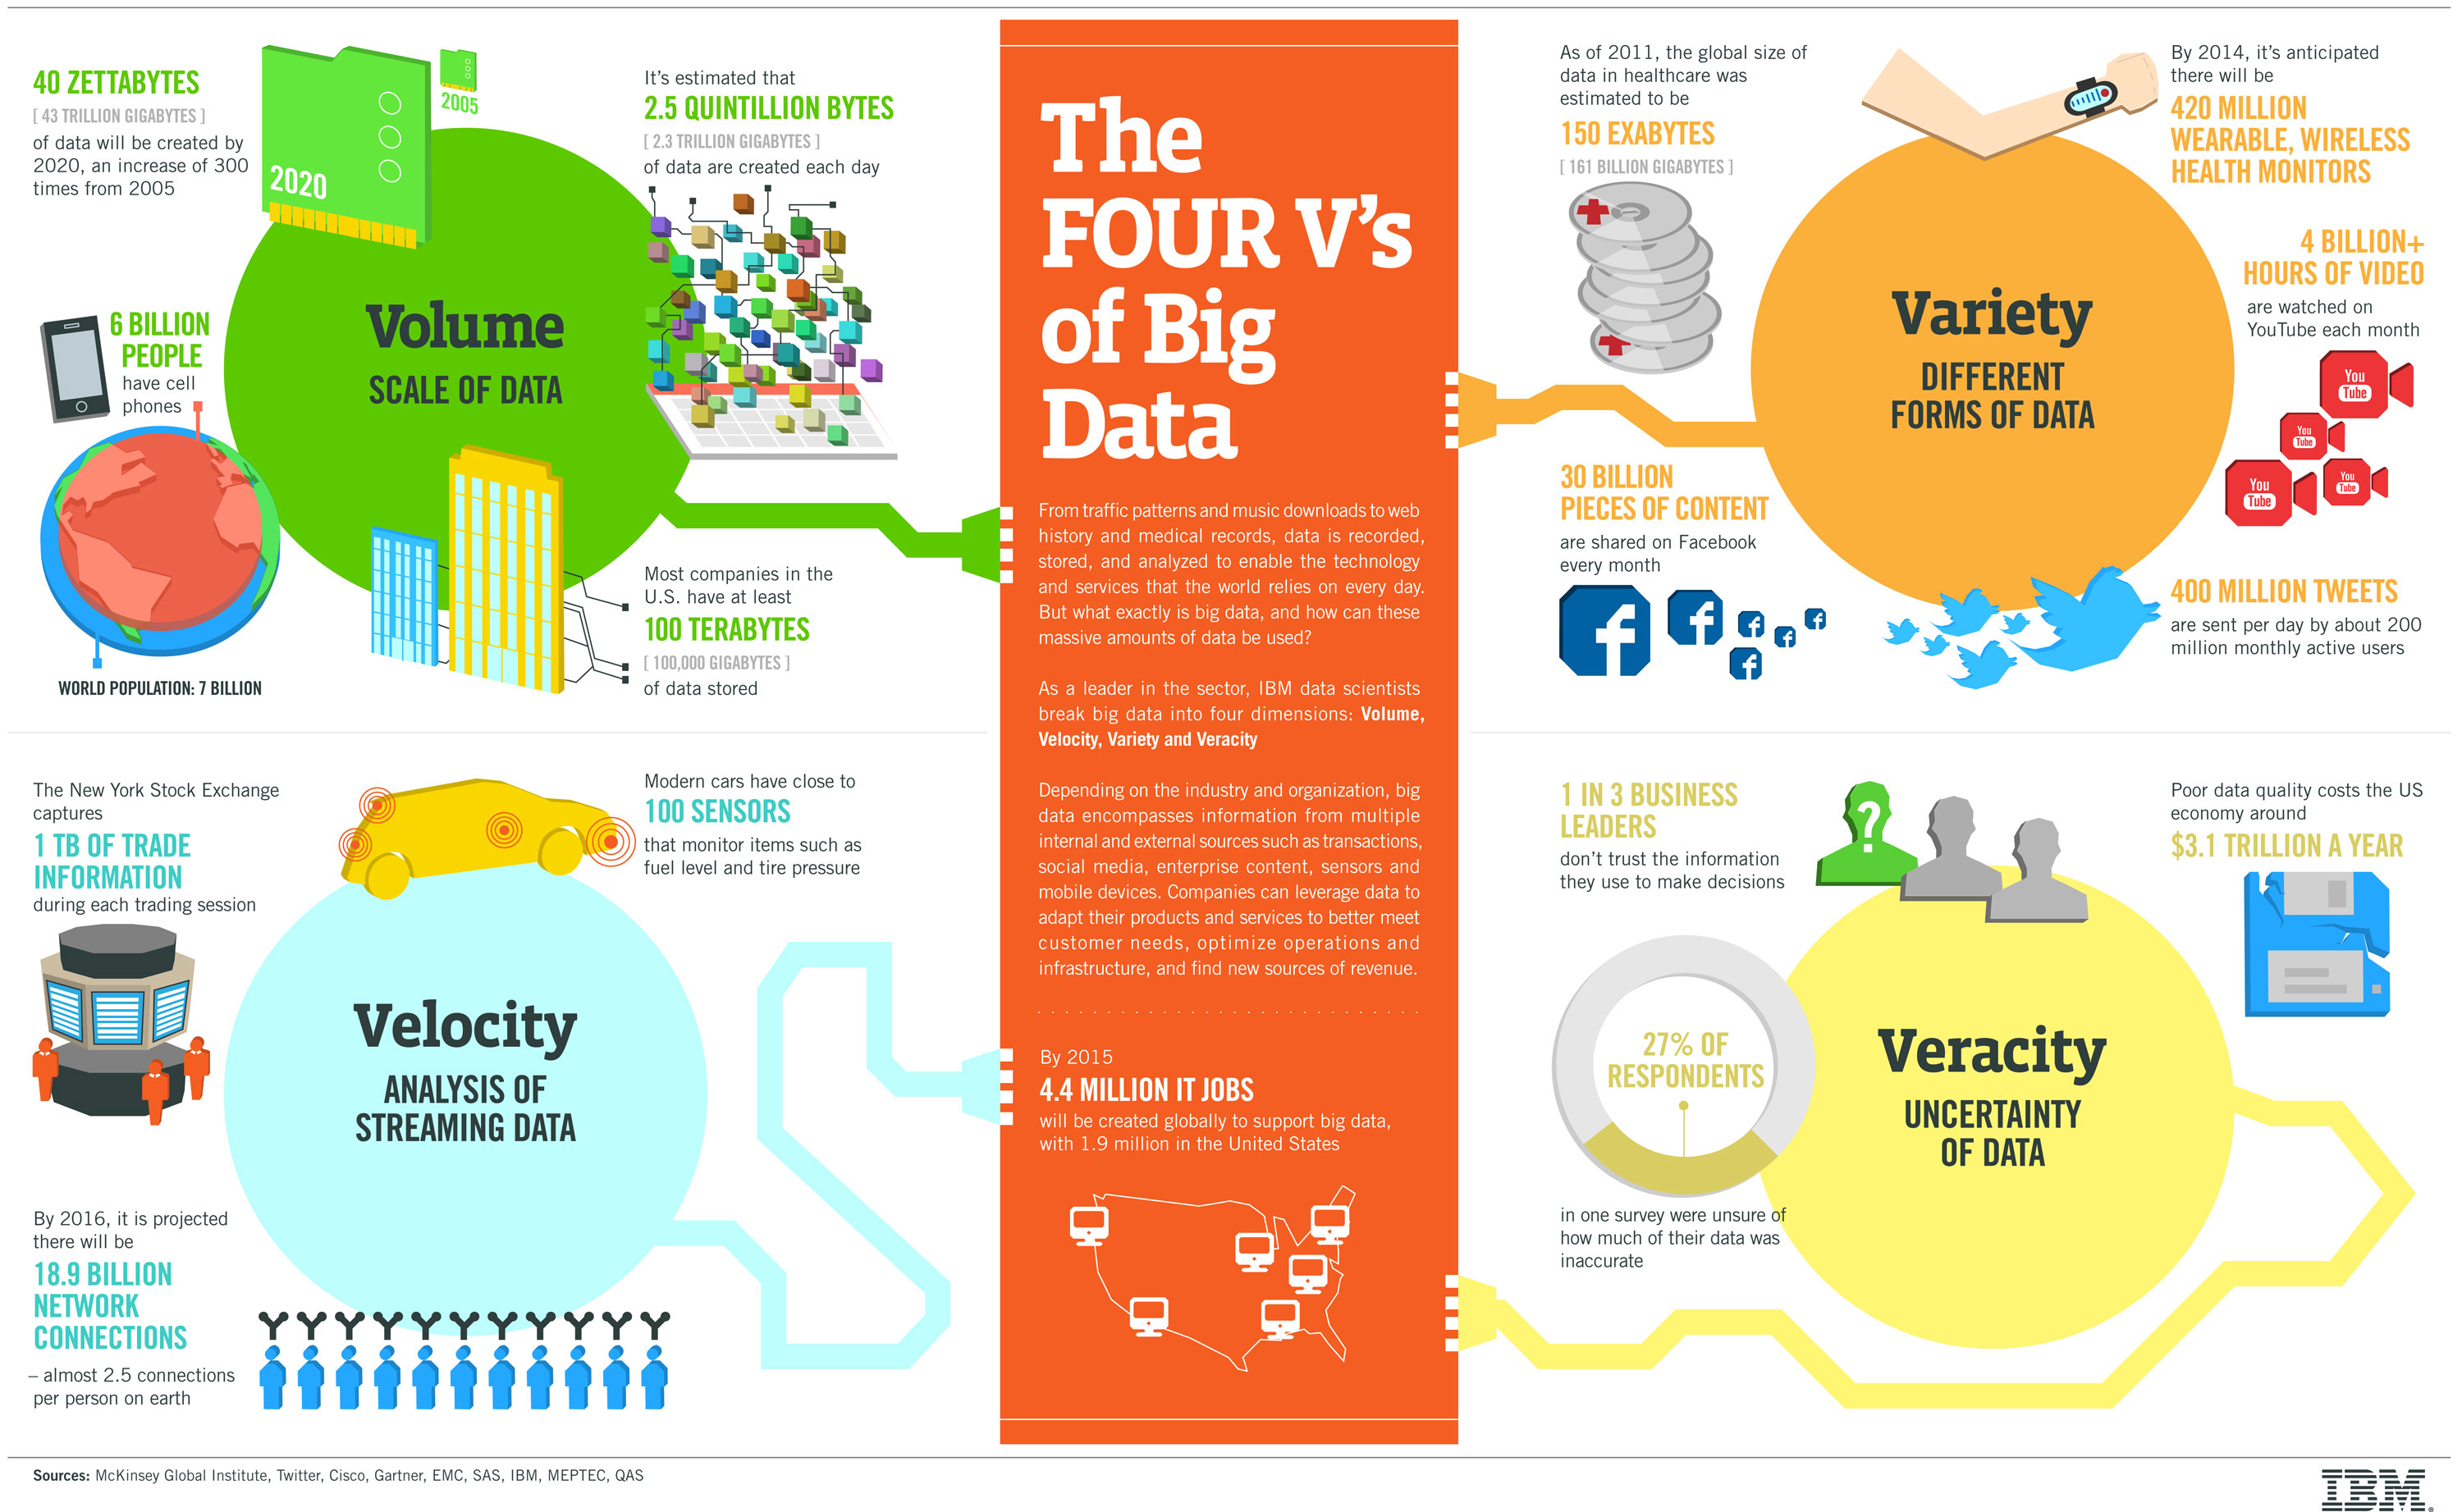
\includegraphics[width=\textwidth]{4-Vs-of-big-data}
% % \end{frame}

% \begin{frame}
%   \frametitle{Big data considerations}
%   \pause

%   In this course, we will focus on learning and developing the fundamental techniques and algorithms that can applied to big data for the purpose of analyses and model building.\\ \pause

%   \bigskip
  
%   Many of these techniques of interest can be grouped under ``machine learning''.\\ \pause

%   \bigskip
  
%   Where relevant, computing considerations will be discussed and explored.
% \end{frame}

\begin{frame}
  \frametitle{What is machine learning?}

  \begin{center}
    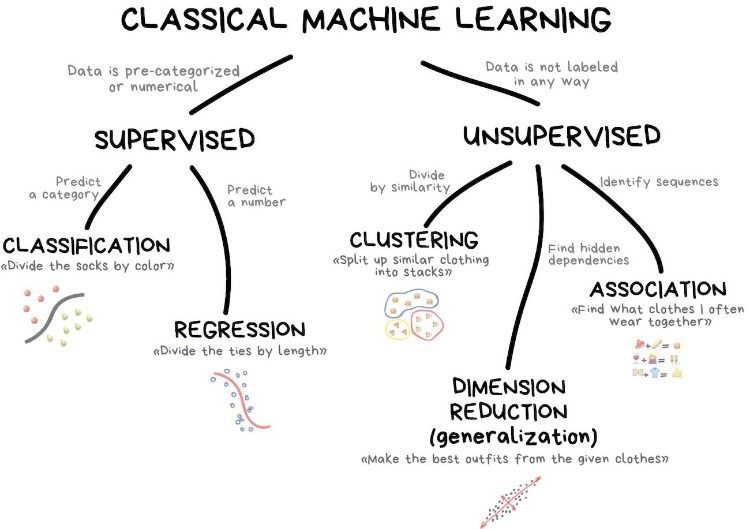
\includegraphics[width=.8\textwidth]{ml_img_1}
  \end{center}
\end{frame}

\begin{frame}
  \frametitle{Machine learning---alternate illustration}

  \begin{center}
    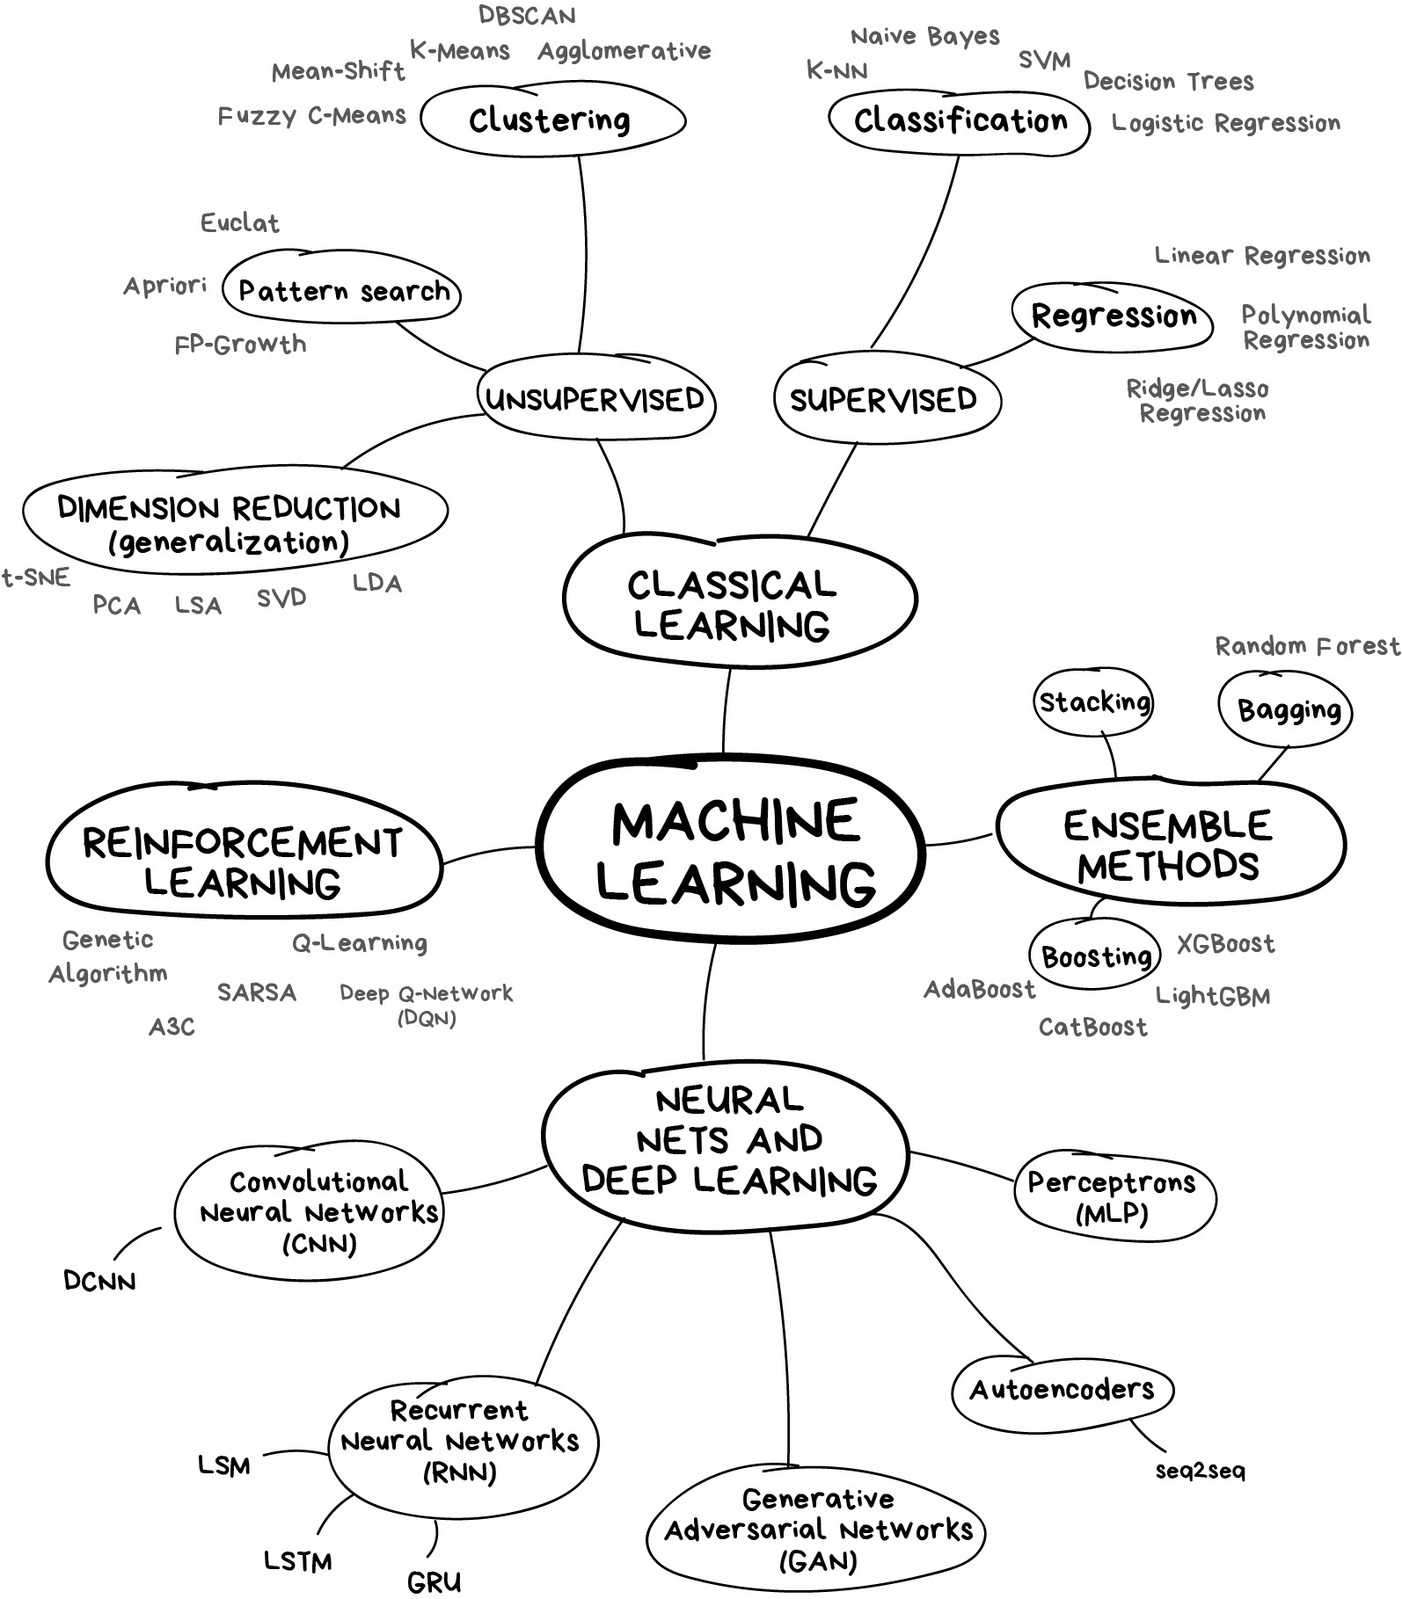
\includegraphics[width=.5\textwidth]{ml_img_2}

    {\tiny Source: \url{https://i.vas3k.ru/7vx.jpg}}
  \end{center}
\end{frame}



\begin{frame}
  \frametitle{Machine learning flow}\pause
  
  The ``learning'' refers to the search for \textbf{optimal parameters} as a function of the data.

  \pause
  
  \begin{itemize}[<+->]
  \item Inputs (data, domain knowledge/human)
  \item Learning (computer/algorithm)
  \item Outputs (predictions, information/inference)
  \end{itemize}

\end{frame}

\begin{frame}
  \frametitle{Supervised vs.\ unsupervised learning}
  \pause
  \begin{minipage}[t]{.45\linewidth}
    \begin{block}{Supervised learning}
      Goal: fit a model characterizing relationship between predictor(s) $X$ and response(s) $Y$ (i.e.\ known outputs)
      \begin{itemize}
      \item regression (linear, nonlinear, logistic, etc)
      \item boosting/bagging/random forests
      \item support vector machines
      \end{itemize}
    \end{block}
  \end{minipage}
  \quad \pause
  \begin{minipage}[t]{.45\linewidth}
    \begin{block}{Unsupervised learning}
      Goal: infer relationships between/among variables or observations (outputs/target unknown)
      \begin{itemize}
      \item dimensionality reduction (principal components, factor analysis)
      \item cluster analysis
      \end{itemize}
    \end{block}
  \end{minipage}
7
  \bigskip
  \pause
  \begin{itemize}
  \item Semi-supervised learning occurs when responses are available for a subset of the observations
  %\item Most neural network problems are supervised (as the responses are known)
  \end{itemize}
\end{frame}

\begin{frame}
  \frametitle{Notation}

  \begin{tabular}[t]{l l}
    \bf Symbol & \bf Meaning \\ \pause
    $n$ & number of observations (distinct data points) \\\pause
    $p$ & number of variables \\\pause
    $x_{ij}$ & value of $j$th variable for $i$th observation \\
  \end{tabular}

  \pause

  \bigskip
   
  So, we can write the $n\times p$ matrix $\bm X$ as:

  \begin{equation*}
    \bm{X} =
    \begin{pmatrix}
      x_{11} & x_{12} & \cdots & x_{1p} \\
      x_{21} & x_{22} & \cdots & x_{2p} \\
      \vdots & \vdots & \ddots & \vdots \\
      x_{n1} & x_{n2} & \cdots & x_{np} \\
    \end{pmatrix}
  \end{equation*}
  \pause

  where the rows of $\bm X$ are: $x_1, x_2, \ldots, x_n$ \\ \pause and the columns are written $\bm x_1, \bm x_2, \ldots, \bm x_p$
\end{frame}

\begin{frame}
  \frametitle{Notation (cont.)}
  We will denote $\bm y$ as the \textit{response} variable vector.

  \pause
  \bigskip
  

  {\bf Summary of notation conventions}

  \begin{itemize}
  \item Scalar: lower case italic (e.g. $b$)
  \item Vector: lower case bold (e.g $\bm x_j \in \mathbb{R}^n$), except for feature vectors of length $p$)
  \item Matrix: upper case bold (e.g. $\bm X \in \mathbb{R}^{n\times p}1$)
  \item Random variable: upper case italic (e.g. $Y\sim \mathcal{N}(\mu,\sigma)$)
  \end{itemize}
  
\end{frame}

\begin{frame}
  \frametitle{Learning framework}
  Given a set of inputs $X_j$ ($j \in \{1, \ldots, p\}$) and a given output $Y$, {\bf \rd ``learning''} refers to the techniques used in estimating the functional relationship between $X_i$ and $Y$ for the purposes of \textit{prediction} and \textit{inference}.\\

  \pause

  \begin{minipage}[t]{.7\linewidth}
    \centering
    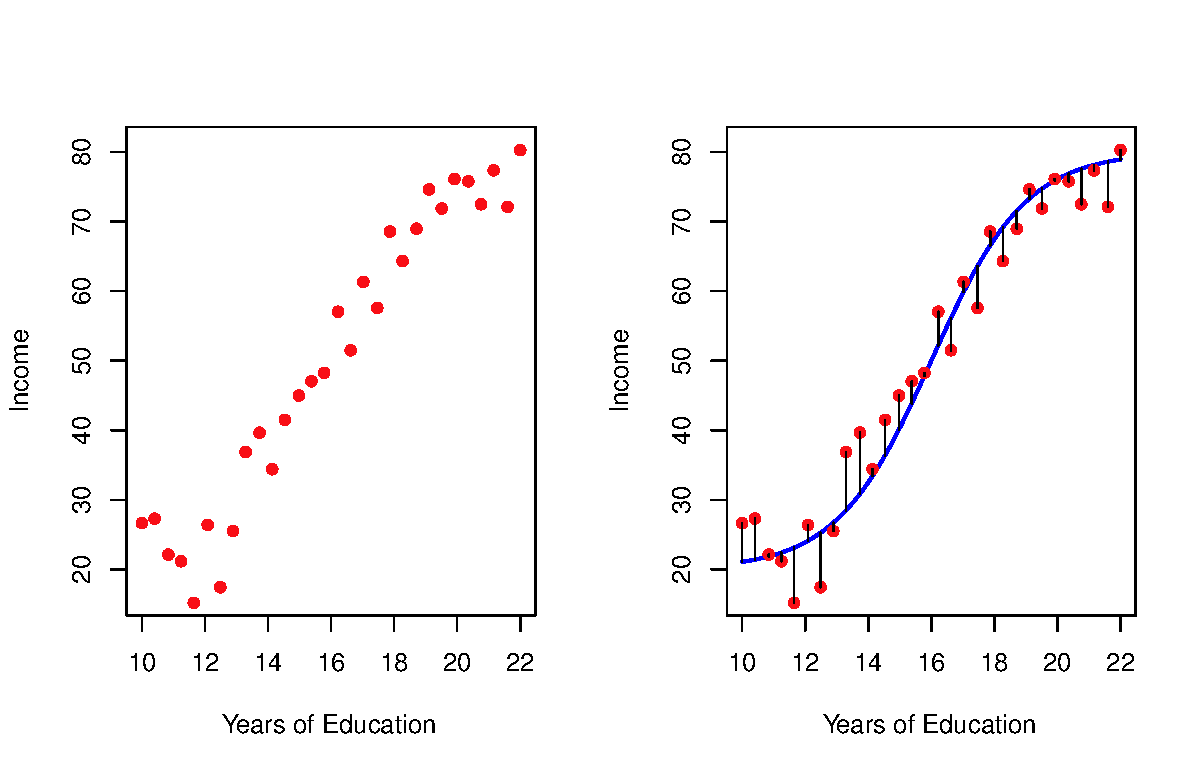
\includegraphics[width=.8\textwidth]{2-2}
  \end{minipage}
  \begin{minipage}[b]{.25\linewidth}
    \begin{figure}[h!]
    \caption{Estimating the functional relationship between income and educational attainment in a data set}
    \label{fig:in}
  \end{figure}
\end{minipage}

  \begin{block}{Model equation}
    \begin{equation}
      \label{eq:3}
      Y = f(X) + \epsilon      
    \end{equation}
    \pause
    where $f$ is an unknown function and $\epsilon$ is the random error (independent of $X$ with zero mean)
  \end{block}

\end{frame}



\begin{frame}
  \frametitle{Prediction}
  We predict $Y$ using:

  \begin{equation}
    \label{eq:0}
    \hat Y = \hat f(X)
  \end{equation}
  \pause

  where $\hat f$ is the estimate of $f$ and $\hat Y$ is the predicted value of $Y$.

  \pause

  \begin{block}{Reducible and irreducible error}
    The prediction accuracy depends on \textit{\bl reducible error} and \textit{\rd irreducible error} (noise---intrinsic variability in the data)
    \begin{align}
      \begin{split}
        E\lt[(Y - \hat Y)^2\rt] &= E\lt[f(X) + \epsilon - \hat f (X))^2\rt] \\
        &= {\bl \lt[f(X) - \hat f(X)\rt]^2 } + {\rd \text{Var}(\epsilon)}
      \end{split}
    \end{align}
  \end{block}
\end{frame}
\begin{frame}
  \frametitle{Inference}
  This refers to the process of determining the nature of the relationship between the inputs $(X)$ and outputs $(Y)$.

  In other words, if $Y = f(X)$, then what is $f$? \pause

  \begin{exampleblock}{Questions relating to inference}
    \begin{itemize}[<+->]
    \item What is the elasticity\footnote{Can be defined as the percentage change in $Y$ for a 1\% change in $X$.} of a certain input in relation to an output?
    \item What are the important \textit{predictors} of a certain outcome?
    \item What is the correlation between $X$ and $Y$?
    \end{itemize}
  \end{exampleblock}
\end{frame}

\begin{frame}
  \frametitle{Parametric methods}
  These methods require an assumption of the structure of the relationship between $X$ and $Y$.

  {\bf \gr Step 1}: assume functional form (e.g. linearity in coefficients):
  \begin{equation}
    \label{eq:1}
    f(X) = \beta_{0} + \beta_{1}X_1 + \beta_2X_2 + \cdots
  \end{equation}

  {\bf \gr Step 2}: fit model, i.e.\ \textit{estimate} the parameters/coefficients:
  \begin{equation}
    \label{eq:2}
    Y \approx  \beta_{0} + \beta_{1}X_1 + \beta_2X_2 + \cdots
  \end{equation}
  The estimation procedure can be a method of choice, e.g. OLS (ordinary least squares), WLS (weighted least squares), etc.
\end{frame}

\begin{frame}
  \frametitle{Non-parametric methods}
  \begin{itemize}
  \item The assumption of linearity is a  strong one and may result in a poor fit if $f$ is very different from $\hat f$.

  \item Non-parametric methods allow flexible functional forms (although the danger of overfitting is real).

  \item For accuracy, however, non-parametric models require many more observations compared to the parametric case.
\end{itemize}
  
\end{frame}

\begin{frame}
  \frametitle{Tradeoff between accuracy and interpretability}\pause

  A simpler model is more interpretable in its parameters. \pause  A highly complicated model may operate more like a blackbox.

  \begin{center}
    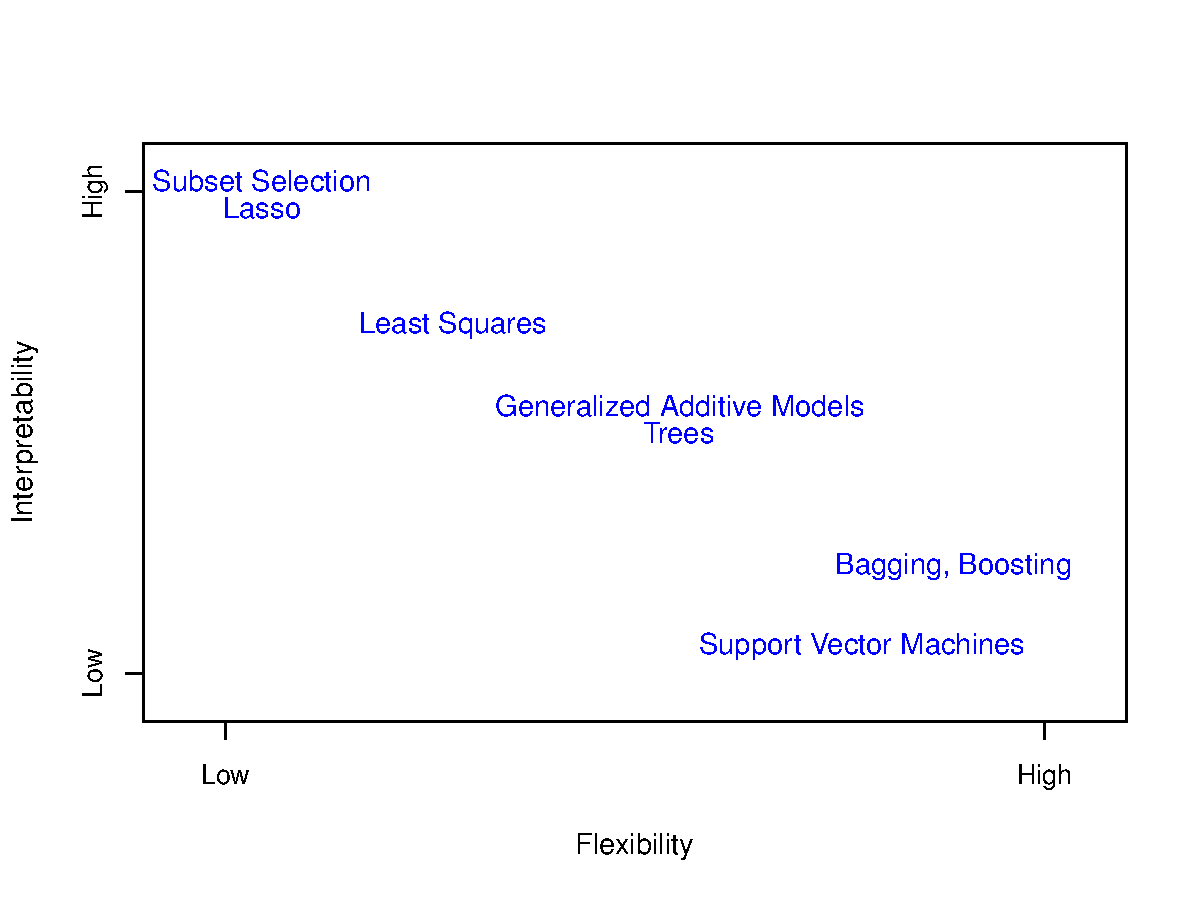
\includegraphics[width=.7\textwidth]{2-7.pdf}
  \end{center}

\end{frame}

\begin{frame}
  \frametitle{Occam's razor}
%    \begin{block}{Occam's Razor}
  \begin{center}
    
\includegraphics[width=.8\textwidth]{occam}
  \end{center}

 % \end{block}

\end{frame}


\section{Basic concepts in probability}

\begin{frame}
  \frametitle{Theory of probability}
  \begin{itemize}[<+->]
  \item Three axioms of probability: 
    \begin{align*}
      P(E) &\ge 0 \quad \text{and} \quad P(E) \le 1 \quad \text{\rd for given event $E$}\\\pause
      P(S) &= 1 \\\pause
      P(E_{1}\cup E_{2}\cup \cdots\cup E_{n}) &= P(E_{1}) + P(E_{2}) + \cdots + P(E_{n})~~ \text{(Mutually exclusive)}
    \end{align*}
  \item Addition rule: $P(A\cup B) = P(A) + P(B) - P(AB)$
    \begin{itemize}[<+->]
    \item For mutually exclusive events: $P(A\cup B) = P(A) + P(B)$ (Axiom 3)
\end{itemize}

  \item Counting events:
    \begin{itemize}[<+->]
    \item Fundamental principle of counting: number of outcomes for $1, \ldots, k$ events, each with $n_{1},\ldots, n_{k}$ possibilities is $\gr n_{1}\times\cdots \times n_{k}$
    \item Permutations (arrangements) of $n$ objects: $\gr n! = n(n-1)(n-2)\cdots(2)(1)$
    \item Permutations of a subset of $k$ items chosen from set of $n$ items: $n!/(n-k)!$
    \item Combinations (distinct; order not important) of group of $k$ items chosen from set of $n$ items: $n!/(k!(n-k)!)$
    \end{itemize}
  \end{itemize}
\end{frame}

\begin{frame}
  \frametitle{Conditional probability}
  \begin{itemize}[<+->]
  \item Conditional probability:\pause
    \begin{equation}
      P(A|B) = \fr{P(AB)}{P(B)}
    \end{equation}

  \item Independent events: \pause
    \begin{equation}
      P(AB) = P(A)P(B)
    \end{equation}

    \item
    Generally, the joint probability (intersection) of any number of independent events is the product of their individual probabilities: \pause
    \begin{equation}
      P(E_{1}\cap E_{2}\cap \cdots \cap E_{n}) = P(E_{1})P(E_{2})\cdots P(E_{n})
    \end{equation}
  \item Multiplication rule:\pause
    \begin{equation}
      P(AB) \pause = P(A|B)P(B)\pause = P(B|A)P(A)
    \end{equation}
  \end{itemize}
\end{frame}

\begin{frame}
  \frametitle{Total probability}

  Useful in situations where the probability of an event cannot be directly
  determined but its conditional probabilities are known.
  
  \pause

  
  \begin{minipage}[b]{.55\linewidth}
    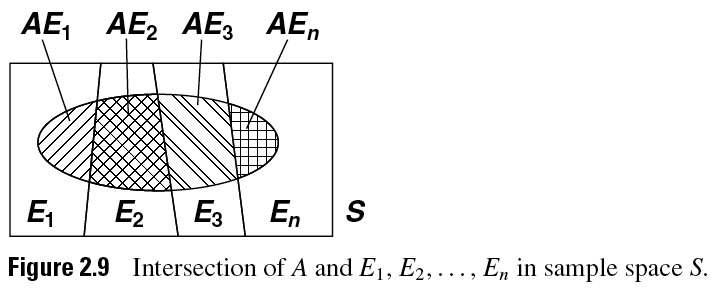
\includegraphics[width=\textwidth,trim={0 1.2cm 11cm 0},clip]{02_09}    
  \end{minipage}\pause\quad
  \begin{minipage}[b]{.35\linewidth}\raggedright
    $P(A)= \pause P(AE_{1}) + \pause P(AE_{2}) $ \pause
    
    \quad\quad\quad $+ \pause P(AE_{3}) + \cdots + P(AE_{n})$  \pause

    \medskip
    
    Note that:\\\pause
    \alert{$P(AE_1) = P(A|E_1)P(E_1)$},\\ etc.
  \end{minipage}
  \pause
  \begin{block}{Theorem of total probability}
    The probability of an event $A$ conditioned on the mutually exclusive and
    collectively exhaustive events $E_1, E_2, \ldots, E_n$ is given by \pause
    \begin{equation}
      \label{eq:19}
      P(A) = P(A|E_1)P(E_1) + P(A|E_2)P(E_2) + \cdots + P(A|E_n)P(E_n)
    \end{equation}
  \end{block}

 
\end{frame}

\begin{frame}
  \frametitle{Derivation of Bayes' theorem} \pause
  
  Recall from the multiplication rule that:\pause
  \begin{equation}
    \label{eq:21}
    P(AB) =   \rd P(A|B)P(B)
  \end{equation}

  \pause

  \medskip
  
  Equivalently: \pause
  \begin{equation}
    \label{eq:22}
    P(AB) =\bl P(B|A)P(A) 
  \end{equation}
  \pause

  We combine both equations to obtain:
  \pause
  \begin{equation}
    \label{eq:23}
   {\rd P(A|B)P(B)} = {\bl P(B|A)P(A)}
  \end{equation}

  \pause

  \medskip
  
  Then, we obtain the \textbf{inverse probability} of the conditioning event:\pause
  \begin{equation}
    \label{eq:24}
    P(B|A) = \fr{P(A|B)P(B)}{P(A)}
  \end{equation}
  \pause

\end{frame}


\begin{frame}
  \frametitle{Bayes' theorem}\pause

  Bayes' Theorem allows for the computation of an inverse probability, e.g. given $P(A|B)$, can we find $P(B|A)$?
  
  \pause
  \begin{block}{}
  \begin{equation}
    \label{eq:25}
    {\pl P(E_i|A)} =\fr{P(A|E_i)P(E_i)}{\sum_{j=1}^{n}P(A|E_j)P(E_j)} = \pause \fr{{\rd P(A|E_i)}{\bl P(E_{i})}}{\gr P(A)}
  \end{equation}
  \pause
  \begin{itemize}[<+->]
  \item {\bf posterior probability: $\pl P(E_i|A)$}
  \item {\bf likelihood: $\rd P(A|E_{i})$}
  \item {\bf prior: $\bl P(E_{i})$}
  \item {\bf evidence (total probability): $\gr P(A)$}
  \end{itemize}
\end{block}

\pause

If the event $A$ can be conditioned on only two events $E_{1}$ and $E_{2}$, then: \pause

\begin{eqnarray}
  P(E_{1}|A) &=& \pause \fr{P(A|E_{1})P(E_{1})}{P(A|E_{1})P(E_{1}) + P(A|E_{2})P(E_{2}) } \\[2mm] \pause
  P(E_{2}|A) &=& \pause \fr{P(A|E_{2})P(E_{2})}{P(A|E_{1})P(E_{1}) + P(A|E_{2})P(E_{2}) } 
\end{eqnarray}
\end{frame}

\begin{frame}
  \frametitle{Example 1: Construction supplies}
    Aggregates for the construction of a reinforced concrete building are supplied by two companies. \pause
    Company $a$ delivers 600 truckloads a day while Company $b$ delivers 400 truckloads a day. \pause
    From prior experience, 3\% of Company $a$'s material is expected to be substandard while 1\% of Company $b$'s material is expected to be susbstandard.\\ \pause

    We define: \pause

    \begin{eqnarray*}
      A &=& \text{aggregates supplied by Company $a$} \\\pause
      B &=& \text{aggregates supplied by Company $b$} \\\pause
      E &=& \text{aggregates are substandard} 
    \end{eqnarray*}

      \begin{enumerate}[a]
  \item Draw a Venn diagram and convince yourself that $P(A) = 0.60, P(B) = 0.40, P(E|A) = 0.03, P(E|B) = 0.01$ \pause
    \item Find the probability $P(A|E) = 0.82$.

      \end{enumerate}
\end{frame}


\begin{frame}
  \frametitle{Example 1: Construction supplies (cont.)}
  \pause
  
  \begin{enumerate}[a]
  \item Draw a Venn diagram and convince yourself that $P(A) = 0.60, P(B) = 0.40, P(E|A) = 0.03, P(E|B) = 0.01$ \pause

    \bigskip
    
    \begin{center}
      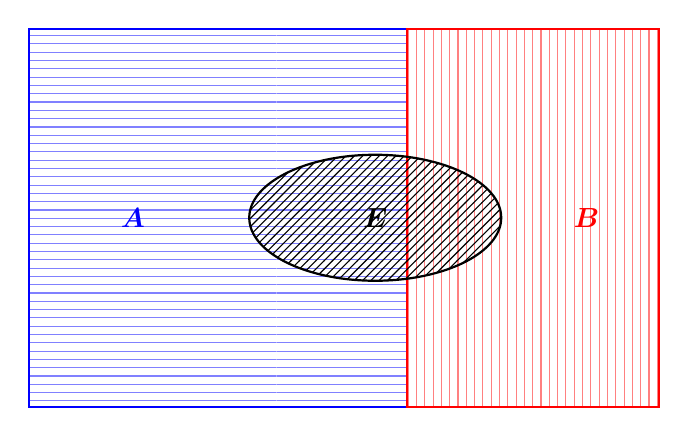
\begin{tikzpicture}[scale=.8]
        \visible<+->{
          \draw[thick,blue, pattern=horizontal lines, pattern color=blue!50!]  (0, 0) rectangle (6,6);
          \node[blue,left] at (2,3) {$\bm A$};
        } % node[anchor=north east, right] {$\bm S$};}
        \visible<+->{
          \draw[thick, red, pattern=vertical lines, pattern color=red!50!]  (6, 0) rectangle (10,6);
          \node[red,right] at (8.5,3) {$\bm B$};
        } 
        \visible<+->{
          \draw[thick,black, pattern=north east lines, pattern color=black] (5.5,3) ellipse (2 cm and 1 cm) node[black] {$\bm E$};
        }

      \end{tikzpicture}
    \end{center}  
    
  \end{enumerate}
\end{frame}

\begin{frame}
  \frametitle{Example 1: Construction supplies (cont.)}\pause

  \[P(A) = 0.60, P(B) = 0.40, P(E|A) = 0.03, P(E|B) = 0.01\]\pause
  
  \begin{enumerate}[a]
  \item $P(E|A) = \frac{P(EA)}{P(A)}$
    \pause
    \begin{center}
      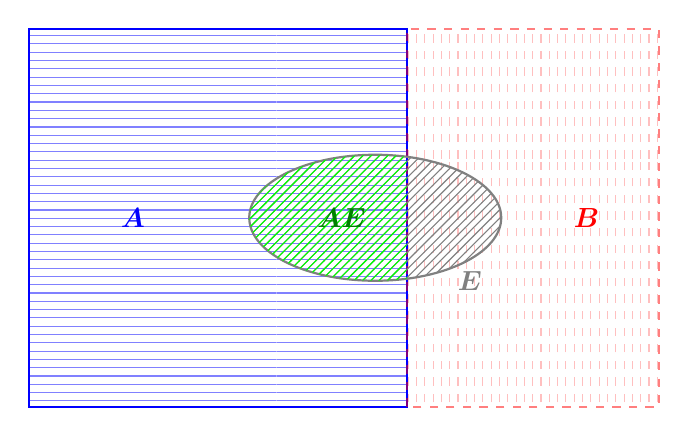
\begin{tikzpicture}[scale=.8]
        \visible<+->{
          \draw[thick,blue, pattern=horizontal lines, pattern color=blue!50!]  (0, 0) rectangle (6,6);
          \node[blue,left] at (2,3) {$\bm A$};
        } % node[anchor=north east, right] {$\bm S$};}
        \visible<+->{
          \draw[dashed,opacity=.5,thick, red, pattern=vertical lines, pattern color=red!50!]  (6, 0) rectangle (10,6);
          \node[red,right] at (8.5,3) {$\bm B$};
        } 
        \visible<+->{
          \draw[gray,thick, pattern=north east lines, pattern color=gray] (5.5,3) ellipse (2 cm and 1 cm);
          \node[gray] at (7,2) {$\bm E$};
        }
        
        % \visible<8->{
        % \fill[white] (-1,0) ellipse (3 cm and 1 cm) ;
        % \fill[white] (3,0) ellipse (4 cm and 1 cm) ;
        % \fill[draw,pattern=north east lines,pattern color=green!50!black]
        % (-1,0) ellipse (3 cm and 1 cm) node[left] {$\bm{P(E_{1})}$};
        % }
        
          \visible<+->{        
          \begin{scope}%[even odd rule]
            \clip (0, 0) rectangle (6,6);
            \fill[green!80!black,pattern=north east lines, pattern color=green] (5.5,3) ellipse (2 cm and 1 cm) node[green!50!black,left]
            {$\bm {AE}$};
           % \node at (4,0)  {$\bm{P(E_{2}) -  P(E_{1}E_{2})}$};
          \end{scope}
          %\draw[] (-1,0) ellipse (3 cm and 1 cm) ;
          %\draw[]  (3,0) ellipse (4 cm and 1 cm);
        }

      \end{tikzpicture}
    \end{center}
  \end{enumerate}
\end{frame}


\begin{frame}
  \frametitle{Example 1: Construction supplies (cont.)}\pause

  \[P(A) = 0.60, P(B) = 0.40, P(E|A) = 0.03, P(E|B) = 0.01\]\pause
  
  \begin{enumerate}[a]
  \item $P(E|B) = \frac{P(EB)}{P(B)}$
    \pause
    \begin{center}
      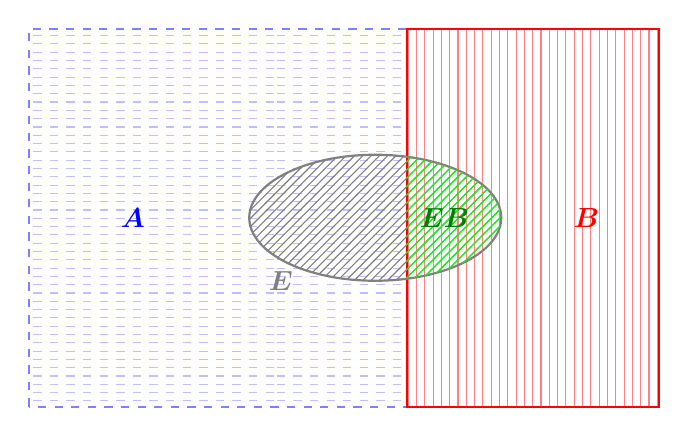
\begin{tikzpicture}[scale=.8]
        \visible<+->{
          \draw[dashed,opacity=.5,thick,blue, pattern=horizontal lines, pattern color=blue!50!]  (0, 0) rectangle (6,6);
          \node[blue,left] at (2,3) {$\bm A$};
        } % node[anchor=north east, right] {$\bm S$};}
        \visible<+->{
          \draw[thick, red, pattern=vertical lines, pattern color=red!50!]  (6, 0) rectangle (10,6);
          \node[red,right] at (8.5,3) {$\bm B$};
        } 
        \visible<+->{
          \draw[gray,thick, pattern=north east lines, pattern color=gray] (5.5,3) ellipse (2 cm and 1 cm);
          \node[gray] at (4,2) {$\bm E$};
        }
        \visible<+->{        
          \begin{scope}%[even odd rule]
            \clip (6, 0) rectangle (10,6);
            \fill[green!80!black,pattern=north east lines, pattern color=green] (5.5,3) ellipse (2 cm and 1 cm);
            \node[green!50!black] at (6.6,3)  {$\bm {EB}$};
          \end{scope}
        }

      \end{tikzpicture}
    \end{center}
  \end{enumerate}
\end{frame}

   
\begin{frame}
  \frametitle{Example 1: Construction supplies (cont.)}

    \begin{enumerate}[a]\setcounter{enumi}{1}
    \item Find the probability $P(A|E) = 0.82$.

      \bigskip
      \pause
      First, we find the evidence: \pause
      {\gr
        \begin{eqnarray*}
         P(E) &=& P(E|A)P(A) + \pause P(E|B)P(B) \\ \pause
              &=& (0.03)(0.6) + \pause (0.01)(0.4) \\ \pause
              &=& 0.018 + \pause 0.004 = 0.022
       \end{eqnarray*}
     }
     
      Then we use Bayes': \pause

      \begin{eqnarray*}
        P(A|E) &=& \fr{\bl P(E|A)P(A)}{{\bl P(E|A)P(A)} + P(E|B)P(B)} \\\pause
               &=& \fr{P(E|A)P(A)}{\gr P(E)} \quad \text{\gr (Denominator: total probability)} \\ \pause
               &=& \fr{{\bl 0.03} \times {\rd 0.60}}{\gr 0.022} \pause \equiv 
                   \fr{ {\bl \text{likelihood}} \times \text{\rd prior}}{\gr \text{evidence}} \\ \pause
               &=& 0.818 \approx \boxed{0.82}
      \end{eqnarray*}
      \pause

      $P(A|E)$ is the posterior probability of $A$ having observed $E$. In other words, having prior knowledge of $A$
      (i.e. $P(A)$ and the likelihood of of $E$ given $A$, we can update our knowledge of $A$ (posterior probability)
      based on these observations.
    \end{enumerate}
 \end{frame}



 \section{Random variables}
 \begin{frame}
  \frametitle{Random variables}\pause

  A random variable is a function that uniquely maps events in a sample space to the set of real numbers. \\ \pause

  \bigskip
  
  A random variable $X$ may be: \pause

  \bigskip
  
  \begin{itemize}
  \item {\it Discrete}
  \item {\it Continuous}
  \item {\it Mixed} (probability defined over both discrete and range of continuous values)
  \end{itemize}
  
\end{frame}
 

 \begin{frame}
  \frametitle{Probability mass function (PMF)}\pause
  \begin{minipage}{.45\linewidth}
  The PMF is given by \pause

  \begin{equation}
    \label{eq:12}
    p_X(x_i) \equiv P(X = x_i) \quad \forall x
  \end{equation}

  \pause
  
  \begin{alertblock}{CDF of discrete random variable}
    \pause
    \begin{align*}
      \label{eq:14}
      F_X(x) &= \sum_{x_i \le x} P(X = x_i)\\
             &= \sum_{x_i \le x}p_X(x_i)
    \end{align*}
  \end{alertblock}
  \end{minipage}\qquad \pause
  \begin{minipage}{.45\linewidth}
    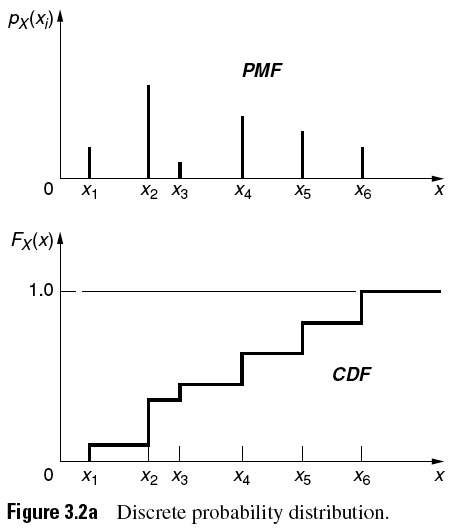
\includegraphics[width=\textwidth, trim={0 1cm 0 0}, clip]{03_02a}
  \end{minipage}
  
  \pause

  \bigskip
  
  The probability masses in a PMF sum up to 1.
\end{frame}

\begin{frame}
  \frametitle{Probability density function (PDF)}\pause

  \begin{minipage}{.45\linewidth}
  The PDF is denoted $f_X(x)$ such that the probability of $X$ in the interval $(a,b]$ is: \pause

  \begin{equation}
    \label{eq:10}
    P(a< X \le b) = \int_a^b f_X(x)dx
  \end{equation}

  \pause
  
  \begin{alertblock}{CDF of continuous random variable}
    \pause
    \begin{align*}
      \label{eq:15}
      F_X(x) &=  P(X \le x)\\
             &= \int_{-\infty}^x f_X(\tau)d\tau
    \end{align*}
  \end{alertblock}

    \pause

    It follows that the PDF is the derivative of the CDF:

    \begin{equation}
      \label{eq:15}
      f_X(x) = \fr{dF_X(x)}{dx}
    \end{equation}
  \end{minipage}
  \begin{minipage}{.45\linewidth}
    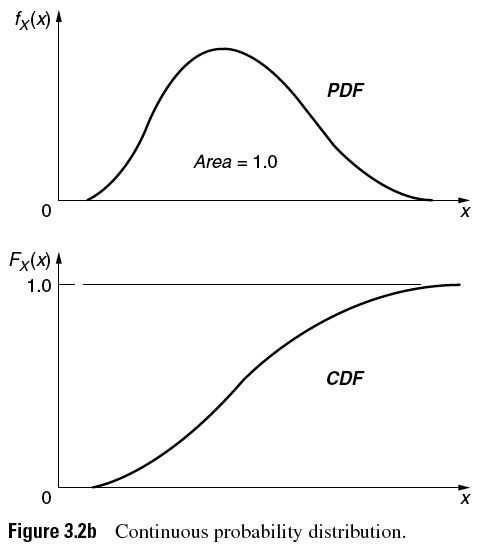
\includegraphics[width=\textwidth, trim={0 2cm 0 0}, clip]{03_02b}
    
  \pause  
  The total area under a PDF is 1.
\end{minipage}

\end{frame}

\begin{frame}
  \frametitle{Central values} \pause
  These include the mean, median and mode. \pause

  \begin{itemize}[<+->]
  \item Mean: weighted average (by probability of occurence) or expected value \pause
    \begin{eqnarray}
      \mathbb{E}(X) = \mu_{X} \pause &=& \sum_i x_i p_X(x_i) \pause \quad \text{\og discrete case}\\ \pause
      \mathbb{E}(X) = \mu_{X} \pause &=& \int_{-\infty}^{\infty}xf_X(x)dx \pause \quad \text{\og continuous case}
    \end{eqnarray}
  \end{itemize}
  \pause
 
  \begin{block}{Generalized expectation} \pause
  The mathematical expectation can be defined for a function $g$ of random variable $X$:\pause
     \begin{align}
      \mathbb{E}[g(X)] &= \sum_i g(x_i) p_X(x_i) \quad \text{\og discrete case}\\ \pause
      \mathbb{E}[g(X)] &= \int_{-\infty}^{\infty}g(x)f_X(x)dx \quad \text{\og continuous case}
    \end{align}
  \end{block}
\end{frame}

 
\begin{frame}
  \frametitle{Measures of dispersion} \pause
  \begin{block}{Variance}\pause
    In  discrete case: \pause
    \begin{equation}
      \label{eq:var}
      \mathbb{V}(X) = \sum_i(x_i - \mu_X)^2p_X(x_i)
    \end{equation}
    \pause

    In  continuous case:\pause
    \begin{equation}
      \label{eq:2}
      \mathbb{V}(X) = \int_{-\infty}^{\infty}(x - \mu_X)^2 f_X(x)dx
    \end{equation}
    \pause

    Expanding both equations results in:
    
    \begin{equation}
      \label{eq:3}\rd
      \mathbb{V}(X) = \mathbb{E}(X^2) - \mu_X^2 \pause = \mathbb{E}(X^{2}) - \mathbb{E}(X)^{2}
    \end{equation}
  \end{block}
\end{frame}



\begin{frame}
  \frametitle{Measures of dispersion (cont.)}
  \pause

  \begin{block}{Standard deviation}
    \pause

    The standard deviation is convenient as it has the same unit as the random variable:\pause

    \begin{equation}
      \label{eq:4}
      \sigma_X = \pause \sqrt{\mathbb{V}(X)}
    \end{equation}
  \end{block}
  
  \pause

  \begin{block}{Coefficient of variation}
    The COV gives the deviation relative to the mean. It is unitless.\pause

    \begin{equation}
      \label{eq:5}
      \delta_X = \frac{\sigma_X}{\mu_X}
    \end{equation}
  \end{block}
  
\end{frame}


\begin{frame}
  \frametitle{Mean of a linear function}\pause
  For a continuous random variable $X$, the mean is defined as\pause
  \begin{equation}
    \label{eq:30}
    \mathbb{E}(X) = \int_{-\infty}^\infty xf_X(x) dx
  \end{equation}
  \pause
  
  Now, given that $Z = aX + bY$, then the mean of $Z$ is\pause
  \begin{eqnarray*}
    \mathbb{E}(Z) &=& \int_{-\infty}^\infty\int_{-\infty}^\infty (aX + bY)f_{X,Y}dxdy \\\pause
         &=& a {\rd \int_{-\infty}^\infty x f_X(x)dx } +  b {\bl \int_{-\infty}^\infty y f_Y(y)dy }\\\pause
         &=& a\mathbb{E}(X) + b\mathbb{E}(Y)
  \end{eqnarray*}
\end{frame}

\begin{frame}
  \frametitle{Variance of a linear function}
  \pause
  We also recall the variance of an r.v.\ $X$:
  \begin{equation}
    \label{eq:31}
    \mathbb{V}(X) = \mathbb{E}[(X - \mu_X)^2]
  \end{equation}
  \pause
  Thus, for $Z = aX + bY$:\pause
  \begin{eqnarray*}
    \mathbb{V}(Z) &=& \mathbb{E}[((aX + bY) - (a\mu_X + b\mu_Y))^2] \\\pause
           &=& \mathbb{E}[(a(X - \mu_X) + b(Y - \mu_Y))^2] \\\pause
           &=& \mathbb{E}[{\rd a^2(X - \mu_X)^2} + {\og  2ab(X - \mu_X)(Y - \mu_Y) } + {\bl b^2(Y - \mu_Y)} ]\\\pause
           &=& {\rd a^2\mathbb{V}(X)} + {\bl b^2\mathbb{V}(Y) } + {\og 2ab Cov(X,Y)}
  \end{eqnarray*}
\end{frame}

\begin{frame}
  \frametitle{Moments}
  \pause
  The $m$-th order moment of a distribution is given by: \pause
  \begin{equation}
    \mathbb{E}(X^{m}) =
    \begin{cases}
      \sum_{i}x_{i}^{m} \cdot p_{X}(x_{i}) & \quad \text{(discrete)} \\[2mm] \pause
      \int x^{m}\cdot f_{X}(x) dx & \quad \text{(continuous)}
    \end{cases}
  \end{equation}
  \pause

  \begin{itemize}[<+->]
  \item $m$-th central moment: $\mathbb{E}[(X - \mu_{X})^{m}]$
  \item Normalized $m$-th central moment: $\lt(\fr{\mathbb{E}[(X-\mu_{X})^{m}]}{\sigma^{m}}\rt)$
  \end{itemize}
  \pause

  \begin{exampleblock}{Examples}\pause
    \begin{itemize}
    \item \textbf{Mean}: first moment, \pause $\mathbb{E}(X)$ \pause
    \item \textbf{Variance}: second central moment, \pause $\mathbb{E}[(X-\mu_{X})^{2}]$\pause
    \item \textbf{Skewness}: normalized third central moment, \pause $\lt(\fr{\mathbb{E}[(X-\mu_{X})^{3}]}{\sigma^{3}}\rt)$
    \end{itemize}
  \end{exampleblock}
\end{frame}



\begin{frame}
  \frametitle{Covariance and correlation}
  Recall that the variance of an r.v.\ $X$ is given by:
  \begin{equation}
    \label{eq:52}
    \mathbb{V}(X) = \mathbb{E}[(X-\mu_X)^2 ] = \mathbb{E}(X^2) - \mathbb{E}(X)^2
  \end{equation}

  Then given two r.v.'s $X$ and $Y$, the {\it covariance} measures the strength of the linear relationship between them.
  \pause
  
  \begin{block}{Covariance}
    \begin{equation}
      \label{eq:50}
      Cov(X,Y) = \mathbb{E}[(X-\mu_X)(Y-\mu_Y)] = \mathbb{E}(XY) - \mathbb{E}(X)\mathbb{E}(Y)
    \end{equation}    
  \end{block}

\pause

  \begin{block}{Correlation coefficient}
    This is the normalized covariance
    \begin{equation}
    \label{eq:51}
    \rho = \fr{Cov(X,Y)}{\sigma_X\sigma_Y}
  \end{equation}
  \end{block}
    
\end{frame}

\begin{frame}
  \frametitle{Joint distributions}\pause
  Given two random variables $X$ and $Y$:

  \begin{block}{Discrete case}
    The joint PMF is:
    \begin{equation}
      \label{eq:62}
      p_{X,Y}(x_i,y_j) = P(X=x_i, Y = y_j)
    \end{equation} \pause
    The CDF is:
    \begin{equation}
      \label{eq:63}
      F_{X,Y}(x,y) = \sum_{x_i \le x}\sum_{y_j \le y} p_{X,Y}(x_i, y_j)
    \end{equation}
  \end{block}
  \pause

  \begin{block}{Continuous case}\pause
    The joint probability is given by:
    \begin{equation}
      P(a < X \le b, c < Y \le d) = \int_a^b \int_c^d f_{X,Y}(x,y)dy dx
    \end{equation}
  \end{block}
\end{frame}




\begin{frame}
  \frametitle{Conditional distributions of continuous random variables}
  Recall the definition of conditional probability (multiplication rule):\pause
  \begin{eqnarray}
    P(A|B) &=& \fr{P(AB)}{P(B)} \\\pause
    P(AB) &=& \pause P(A|B)P(B)  = \pause P(B|A)P(A)
  \end{eqnarray}
  \pause
  Similarly, for two continuous r.v.'s, the conditional PDF of $X$ given $Y$ is:
  \begin{equation}
    \label{eq:10}
    f_{X|Y}(x|y) = \fr{f_{X,Y}(x,y)}{f_Y(y)}
  \end{equation}
  \pause
  \begin{block}{Joint PDF and CDF of two variables}\pause
  The joint PDF is given by:
  \begin{equation}
    \label{eq:11}
    f_{X,Y}(x,y) = f_{X|Y}(x|y)f_Y(y) = f_{Y|X}(y|x)f_X(x)
  \end{equation}
  \pause
  While the joint CDF is given by:
   \begin{equation}
    \label{eq:13}
    F_{X,Y}(a,b) = P(X\le a,Y\le b) =\pause \int_{-\infty}^a \int_{-\infty}^b f_{X,Y}(x,y)dydx
  \end{equation}
\end{block}
\end{frame}

\begin{frame}
  \frametitle{Marginal distributions of continuous random variables} \pause
  Recall the theorem of total probability:\pause
  \begin{equation}
    \label{eq:12}
    P(A) = \pause \sum_{i=1}^n \pause P(A|E_i) \pause P(E_i)
  \end{equation}
  \pause
  Similarly, the marginal PDFs from a joint distribution of two continuous r.v.'s $X$ and $Y$ is given as:\pause
  \begin{eqnarray}
    f_X(x) &=& \pause \int_{-\infty}^\infty f_{X|Y}(x|y)f_Y(y)dy =\pause \int_{-\infty}^\infty f_{X,Y}(x,y)dy \\ \pause
    f_Y(y) &=&\pause \int_{-\infty}^\infty f_{Y|X}(y|x)f_X(x)dx =\pause  \int_{-\infty}^\infty f_{X,Y}(x,y)dx
  \end{eqnarray}
\end{frame}

% \begin{frame}
%   \frametitle{Example 2: Water levels}\pause
%     The daily water levels of two reservoirs A and B are denoted by two r.v.'s $X$ and $Y$ having the following joint PDF:\pause
%     \begin{equation*}
%       f(x,y) = \fr65\lt(x  + y^2\rt), \quad 0 < x < 1; 0 < y< 1
%     \end{equation*}
%     \pause
%     \begin{enumerate}[(a)]
%     \item Determine the marginal density function of the daily water level for reservoir A.
%     \item If reservoir A is half full on a given day, what is the probability that the water level for reservoir B  will be more than half full?
%     \end{enumerate}
%  \end{frame}

% \begin{frame}
%   \frametitle{Example 2: Water levels (cont.)}\pause
%       \begin{equation*}
%       f(x,y) = \fr65\lt(x  + y^2\rt), \quad 0 < x < 1; 0 < y< 1
%     \end{equation*}
    
%   \begin{exampleblock}{Solution}
%     \begin{enumerate}[a]
%     \item We obtain the marginal density function $f_X(x)$ by integrating the joint PDF over $y$:\pause
%       \begin{eqnarray*}
%         f_X(x) &=& \int_0^1\fr65\lt(x+y^2\rt)dy  \\\pause
%                &=& \fr65\lt[xy + \fr{y^3}{3}\rt]_0^1 \\\pause
%                &=& \fr25\lt(3x + 1\rt) \quad (0 < x < 1)
%       \end{eqnarray*}
%     \end{enumerate}
%   \end{exampleblock}

%     \pause

%     This is the \textbf{marginal distribution}
%  \end{frame}


% \begin{frame}
%   \frametitle{Example 2: Water levels (cont.)}\pause

%   \begin{equation*}
%     f(x,y) = \fr65\lt(x  + y^2\rt), \quad 0 < x < 1; 0 < y< 1
%   \end{equation*}
  
%   \begin{exampleblock}{Solution}
%     \begin{enumerate}[a]\setcounter{enumi}{1}
%     \item {\gr If reservoir A is half full on a given day, what is the probability that the water level in B will be more than half full?} \pause
%       We first find the conditional distribution:\pause
%       \begin{eqnarray*}
%         f_{Y|X}(y|x) &=& \fr{f_{X,Y}(x,y)}{f_X(x)} = \pause \fr{\fr65\lt(x+y^2\rt)}{\fr25\lt(3x + 1\rt)} \pause = 3\fr{x+y^2}{3x +1}\\\pause
%         \text{Thus: } P(Y > 0.5 | X = 0.5) &=& \pause \int_{0.5}^1f_{Y|X}(y|x=0.5)dy \\\pause
%                      &=&3\int_{0.5}^1\fr{0.5+y^2}{1.5 + 1} dy \\\pause
%                      &=& \lt(\fr3{2.5}\rt)\pause \lt[0.5y + \fr{y^3}{3}\rt]_{0.5}^1 \pause
%                      = \boxed{\gr 0.65}
%       \end{eqnarray*}
%     \end{enumerate}
%   \end{exampleblock}

%  \end{frame}

\section{Probability distributions}

\begin{frame}
  \frametitle{Bernoulli distribution}
  \pause
  Let $X$ be an event with only two outcomes \{1,0\}. \pause And let the probability of the event be given by:
  \pause
  \begin{equation*}
    p(X) = \theta, \quad 0\le\theta \le1
  \end{equation*}
  \pause
  And $p(X=1) = \theta$ and $p(X=0) = 1-\theta$.
  \pause
  $X$ is said to be Bernoulli distributed:
  \pause
  \begin{equation}
    X \sim \mathrm{Ber}(\theta)
  \end{equation}
  \pause
  The PMF is then given by: \pause
  \begin{equation}
  \mathrm{Ber}(x| \theta) := \theta^x(1 - \theta)^{1-x}
\end{equation}
\end{frame}
\begin{frame}
  \frametitle{Binomial distribution}
    \pause

  Given a Bernoulli sequence with $X$ random number of occurrences of an event, $N$ trials and $\theta$ the probability of occurrence of each event: \pause

  \begin{itemize}[<+->]
  \item  $X\sim \mathrm{Bin}(N, \theta)$ 
  \item    PMF: $ P(X = x) := \pause \mathrm{Bin}(x| N, \theta) \pause := {N \choose x}p^x (1-\theta)^{N-x}, \quad x = 0, 1, 2, \ldots, N$ 
  \item CDF:       $F_X(x) = \pause P(X \le x) = \pause  \sum_{k=0}^{x}{N \choose k}\theta^k (1-\theta)^{N-k}$ 
  \item    Mean: $\mathbb{E}(X) = N \theta$
  \item    Variance: $\mathbb{V}(X) = N \theta (1-\theta)$ 
  \end{itemize}
  \pause

  \begin{center}
      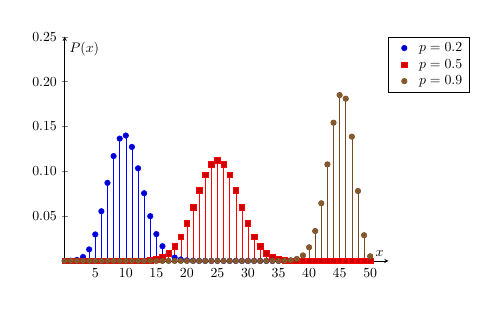
\begin{tikzpicture}[scale = 0.5,
    declare function={binom(\k,\n,\p)=\n!/(\k!*(\n-\k)!)*\p^\k*(1-\p)^(\n-\k);}
    ]
    \begin{axis}[
      samples at={0,...,50},
      xlabel=$x$,
      ylabel=$P(x)$,
      xlabel style={right},
      ylabel style={above left},
      xtick={0,5,...,50},
      ytick={0.05,0.10,...,0.25},
      axis x line=center,
      axis y line=center,
      xmax = 53,
      ymax =.25,
      x post scale=1.2,
      legend style={at={(1.25, 1)},anchor=north east},
      yticklabel style={
        /pgf/number format/fixed,
        /pgf/number format/fixed zerofill,
        /pgf/number format/precision=2
      }
      ]
      \only<+->{\addplot+[ycomb] {binom(x,50,0.2)}; \addlegendentry{$p=0.2$}}
      \only<+->{\addplot+[ycomb] {binom(x,50,0.5)}; \addlegendentry{$p=0.5$}}
      \only<+->{\addplot+[ycomb] {binom(x,50,0.9)}; \addlegendentry{$p=0.9$}} 
    \end{axis}
  \end{tikzpicture}
  \end{center}
\end{frame}

\begin{frame}
  \frametitle{Bernoulli, binomial, categorical and multinomial}
  \begin{itemize}
  \item The Bernoulli distribution is a special case of the binomial distribution with $N = 1$\pause
  \item The categorical distribution is generalization of the Bernoulli to more than two outcomes for a single trial (e.g.\ set of labels $x \in \{1, ..., C\}, C > 2$):
    \pause
    \begin{equation}
      \mathrm{Cat}(\bm x| \bm{\theta}) := \prod_{c=1}^{C} \theta_c^{x_c}
    \end{equation}
    where $\bm x$ is a one-hot vector (e.g. (1,0,0,0) for class 1 of four classes)
    \pause
  \item The multinomial distribution generalizes the categorical distribution for multiple trials: \pause
    \begin{equation}
      \mathscr{M}(\bm{x}| N, \bm{\theta}) := {N \choose {N_1 \ldots N_C}} \prod_{c=1}^C\theta_c^{N_c}
    \end{equation}
  \end{itemize}
\end{frame}
\begin{frame}
  \frametitle{Poisson distribution} \pause
  \begin{itemize}[<+->]
  \item The Poisson distribution is used to model the probability that a number of independent events occur within a fixed time interval (or within a finite space)

  \item Such events are described as Poisson processes

  \item The PMF of a Poisson random variable with {\bf \rd rate parameter $\bm\la$} is given by:\pause
    \begin{equation}
      P(X=x) := \mathrm{Poiss}(x|\la) \pause := \fr{\la^{x}}{x!} e^{-\la}, \quad x \ge 0
    \end{equation}
    \pause

  \item The mean and variance of a Poisson random variable are equal:
    \begin{equation}
      \mathbb{E}(X) = \mathbb{V}(X) = \la
    \end{equation}


  \end{itemize}

  \pause

    \begin{center}
  \begin{tikzpicture}[scale=0.5]
    \begin{axis}[
      axis x line=center,
      axis y line=center,
      xtick={0,2,...,19},
      ytick={0.1,0.2,...,0.4},
      domain = 0:18,
      samples = 19,
      xlabel={$x$},
      ylabel={$P(X=x)$},
      xlabel style={right},
      ylabel style={above left},
      ymax=0.5,
      xmax=20,
      x post scale=1.4
      ]
     \only<7->{\addplot+[ycomb,blue,thick,opacity=.5] {poiss(1))}; \addlegendentry{$\lambda = 1$}}
     \only<8->{\addplot+[ycomb,red,thick,opacity=.5] {poiss(5))};}
     \only<9->{\addlegendentry{$\lambda = 5$}}
     \only<10->{\addplot+[ycomb,brown,thick,opacity=.5] {poiss(9))};}
     \only<11->{\addlegendentry{$\lambda = 9$};}
    \end{axis}
  \end{tikzpicture}
\end{center}
\end{frame}

\begin{frame}
  \frametitle{Gaussian distribution}\pause
  The PDF of a Gaussian (normal) distribution $X \sim \mathscr{N}(\mu, sigma^2)$ is given by:\pause
  \begin{equation}
    \mathscr{N}(x| \mu, \sigma^2) := \fr{1}{\sigma\sqrt{2\pi}} \exp\lt[-\fr12\lt(\fr{x-\mu}{\sigma}\rt)^{2}\rt]
    \end{equation}
    \pause
    where $\mu$ is the mean and $\sigma^2$ is the variance.
    \pause

      \begin{equation}
     P(a < X \le b) = \fr{1}{\sigma\sqrt{2\pi}}\int_a^b e^{-\fr12\lt(\fr{x-\mu}{\sigma}\rt)^2}dx
    =  \Phi\lt(\fr{b-\mu}{\sigma}\rt) -  \Phi\lt(\fr{a-\mu}{\sigma}\rt)
  \end{equation}
  \pause
  where $\Phi$ is the CDF of the standard normal distribution ($ N(0,1)$).

  \pause

  \begin{center}
    \begin{tikzpicture}[scale = 0.5]
    \begin{axis}[no markers, domain=0:10, samples=100,
      axis lines*=left, xlabel=$s$, ylabel=$f_S(s)$,,
      height=6cm, width=10cm,
      xtick={-3, -2, -1, 0, 1, 2, 3}, ytick=\empty,
      enlargelimits=false, clip=false, axis on top,
      grid = major]

      \only<7->{        \addplot [fill=gray, draw=none, domain=-3:3] {gauss(0,1)} \closedcycle;
      }
      
      \only<8->{
        \addplot [fill=cyan!20, draw=none, domain=-1:1] {gauss(0,1)} \closedcycle;
        \node[coordinate, pin={34.1\%}] at (axis cs: -0.5, 0){};
        \node[coordinate, pin={34.1\%}] at (axis cs: 0.5, 0){};}
      
      \only<9->{
        \addplot [fill=blue!20, draw=none, domain=-2:-1] {gauss(0,1)} \closedcycle;
        \addplot [fill=blue!20, draw=none, domain=1:2] {gauss(0,1)} \closedcycle;
        \node[coordinate, pin={13.6\%}] at (axis cs: 1.5, 0){};
        \node[coordinate, pin={13.6\%}] at (axis cs: -1.5, 0){};}

      \only<10->{
        \addplot [fill=orange!20, draw=none, domain=-3:-2] {gauss(0,1)} \closedcycle;
        \addplot [fill=orange!20, draw=none, domain=2:3] {gauss(0,1)} \closedcycle;
        \node[coordinate, pin={2.1\%}] at (axis cs: 2.5, 0){};
        \node[coordinate, pin={2.1\%}] at (axis cs: -2.5, 0){};}
      
      % \addplot[] coordinates {(-1,0.4) (1,0.4)};
      % \addplot[] coordinates {(-2,0.3) (2,0.3)};
      % \addplot[] coordinates {(-3,0.2) (3,0.2)};
      % \node[coordinate, pin={68.2\%}] at (axis cs: 0, 0.4){};
      % \node[coordinate, pin={95\%}] at (axis cs: 0, 0.3){};
      % \node[coordinate, pin={99.7\%}] at (axis cs: 0, 0.2){};



    \end{axis}
  \end{tikzpicture}
\end{center}

\end{frame}
 

 \begin{frame}
  \frametitle{Lognormal distribution}

     A random variable $X$ that is lognormally distributed with the parameters $\mu$ and $\sigma^{2}$ (denoted $X\sim \mathscr{L\!N}(\mu,\sigma^{2}$)
    has the PDF: \pause

    \begin{equation}
      \label{eq:1}
      \mathscr{L\!N}(x|\mu,\sigma^2) = \fr{1}{(\sigma x)\sqrt{2\pi}}\exp\lt[-\fr{1}{2}\lt(\fr{\ln(x)-\mu}{\sigma}\rt)^2\rt] \quad x \ge 0
    \end{equation}
   \pause
  \begin{center}
    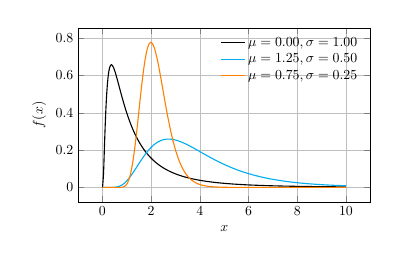
\begin{tikzpicture}[scale = 0.5, declare function = { lognormal(\x,\mu,\sigma)=
        exp(-(ln(x)-\mu)^2/(2*\sigma^2))/(x*\sigma*(2*3.1415)^(0.5)); }]

      \def\parA{\mu} \def\parB{\sigma} \def\va{x}

  \begin{axis}[
    width = 9cm, height = 6cm,
    samples = 250, smooth, domain = -0.2:10,
    xlabel = $\va$, ylabel = $f(\va)$,
    grid=both,
%     xlabel style = {at = {(1,0)}, anchor = north west},
%     ylabel style = {rotate = -90, at = {(0,1)}, anchor = south east},
    legend style = {draw = none, fill = none}, clip = false]

    \only<+->{\addplot[black, thick] {lognormal(x, 0, 1)}; \addlegendentry{$\parA = 0.00, \parB = 1.00$};}

    \only<+->{\addplot[cyan, thick] {lognormal(x, 1.25, 0.5)}; \addlegendentry{$\parA = 1.25, \parB = 0.50$};}

    \only<+->{\addplot[orange, thick] {lognormal(x, 0.75, 0.25)}; \addlegendentry{$\parA = 0.75, \parB = 0.25$};}

    % \node[anchor = south] at (axis description cs: 0.5, 1.05)
    % {$f(\va) = \displaystyle\frac{1}{\va \parB \sqrt{2 \pi}}
    % \exp\left\{-\frac{\left(\ln(\va) - \parA\right)^2}{2 \parB^2}
    % \right\}$};
  \end{axis}
\end{tikzpicture}
\end{center}

\pause

    CDF: $F_{X}(x) = P(X\le x) = \Phi((\ln(x) - \mu)/\sigma)$\\\pause
    Mean: $ \mathbb{E}(X) = e^{\lt(\mu + \fr12 \sigma^2\rt)}$\\
     \pause    
    Variance:
       $\mathbb{V}(X) = \pause   (e^{\sigma^2} - 1)e^{(2\mu + \sigma^{2})}$
     
  
\end{frame}


\begin{frame}
  
  \frametitle{ Exponential distribution}
\pause
  A random variable $X$  exponentially distributed with parameter $\la$ has the PDF:\pause
    \begin{equation}
      \mathrm{Exp}(x|\la) = \pause \la e^{-\la x} \pause \qquad x > 0
    \end{equation}
   \pause

  \begin{center}
      \begin{tikzpicture}[scale=0.6]
      \begin{axis}[no marks, width=10cm, height=5cm,
        samples = 100,
        axis x line=center,
        axis y line=center,
        xtick={0,1,2,...,8},
        ytick={0,0.25,...,2},
        domain = 0:8,
        xlabel={$x$},
        ylabel={$f_X(x)$},
        xlabel style={right},
        ylabel style={above },
        ymax=2.1,
        xmax=8.2,
        %x post scale=1.7,
        enlargelimits=false,
        grid=both,
        yticklabel style={
          /pgf/number format/fixed,
          /pgf/number format/fixed zerofill,
          /pgf/number format/precision=2
        }
        ]
        \addplot+[draw=orange,   thick,opacity=1] {expo(.5,x)}; \addlegendentry{ $\la = 0.5$}
        \addplot+[draw=red,   thick,opacity=1] {expo(1,x)}; \addlegendentry{ $\la = 1.0$}
        \addplot+[draw=green!50!black,   thick,opacity=1] {expo(1.5,x)}; \addlegendentry{ $\la = 1.5$}
        \addplot+[draw=blue,   thick,opacity=1] {expo(2,x)}; \addlegendentry{ $\la = 2.0$}        
%        \addplot+[draw=black,thick, pattern=north east lines, opacity=1, domain=0:1] {expo(1.5,x)} \closedcycle; 
      \end{axis}
    \end{tikzpicture}
\end{center}

\pause
CDF:
    \begin{eqnarray}
       \quad  F_{X}(x) &=& P(X \le x) = \pause  1 - e^{-\la x}, \pause \qquad x > 0 
    \end{eqnarray}

    \pause

    Mean:
    \begin{equation}
      \mathbb{E}(X) = 1/\la
    \end{equation}

    \pause

    Variance:
    \begin{equation}
      \mathbb{V}(X) = 1/\la^{2}
    \end{equation}
 \end{frame}
 

 \begin{frame}
   \frametitle{Multivariate normal distribution (MVN)}
   \pause
   The MVN PDF is given by:\pause
   \begin{equation}
     \mathscr{N}(\bm{x} | \bm{\mu}, \bm{\Sigma}) :=
     \fr{1}{(2\pi)^{D/2}|\bm{\Sigma}|^{1/2}} \exp \lt[ -\fr{1}{2} ({\bm x} - {\bm\mu})^T{\bm\Sigma}^{-1}({\bm x} - {\bm \mu})\rt]
     \end{equation}
     \pause
     where:
     \begin{itemize}
     \item $\bm\mu = \mathbb{E}[{\bm x}] \in \mathbb{R}^D$ is the mean vector \pause
     \item $\bm\Sigma = \mathrm{Cov}[{\bm x}]$ is the $D\times D$ covariance matrix: \pause
       \begin{equation}
         \mathrm{Cov}[{\bm x}] := \mathbb{E}\lt[ (\bm x - \mathbb{E}[{\bm x}])(\bm x - \mathbb{E}[{\bm x}])^T\rt]
       \end{equation}
     \end{itemize}
     \pause
     In 2D:
     \pause
     \begin{equation}
       \bm{\Sigma} =
       \begin{pmatrix}
         \sigma_1^2 & \sigma_{12}^2 \\ \sigma_{21}^2 & \sigma_{2}^2
       \end{pmatrix}
       = \pause
       \begin{pmatrix}
         \sigma_1^2 & \rho\sigma_{1}\sigma_2 \\ \rho\sigma_{1}\sigma_2 & \sigma_{2}^2
       \end{pmatrix}
     \end{equation}
     \pause
     where $\rho$ is the correlation coefficient.
 \end{frame}

\begin{frame}
  \frametitle{Bivariate MVN} \pause

  Marginal distributions: $P(x_1)$ and  $P(x_2)$; \quad \pause
  Joint distribution: $P(x_1,x_2)$. \pause
  
  \pgfplotsset{
    colormap={whitered}{color(0cm)=(white); color(1cm)=(purple!75!blue)}
  }

  \begin{tikzpicture}[scale=.6,
    declare function={mu1=1;},
    declare function={mu2=2;},
    declare function={sigma1=0.5;},
    declare function={sigma2=0.45;},
    declare function={normal(\m,\s)=1/(\s*sqrt(2*pi))*exp(-(x-\m)^2/(2*\s^2));},
    declare function={bivar(\ma,\sa,\mb,\sb)=
      1/(2*pi*\sa*\sb) * exp(-((x-\ma)^2/\sa^2 + (y-\mb)^2/\sb^2))/2;}]
    \begin{axis}[
      colormap name=whitered,
      width=15cm,
      view={45}{65},
      enlargelimits=false,
      grid=major,
      domain=-1:3,
      y domain=-1:5,
      zmax=1,
      samples=26,
      xlabel=$x_1$,
      ylabel=$x_2$,
      zlabel={$P$},
      colorbar,
      colorbar style={
        at={(1.1,0)},
        anchor=south west,
        height=0.25*\pgfkeysvalueof{/pgfplots/parent axis height},
        title={$P(x_1,x_2)$}
      }
      ]
      \only<4->{\addplot3 [domain=-1:3,samples=31, samples y=0, red, thick, smooth] (x,5,{normal(mu1,sigma1)});}
      \only<6->{\addplot3 [domain=-1:5,samples=31, samples y=0, blue, thick, smooth] (-1,x,{normal(mu2,sigma2)});}

      \only<10->{\addplot3 [surf] {bivar(mu1,sigma1,mu2,sigma2)};}

      \only<8->{\draw [black!50] (axis cs:-1,0,0) -- (axis cs:4,0,0);}
      \only<9->{\draw [black!50] (axis cs:0,-1,0) -- (axis cs:0,5,0);}

      \only<7->{\node[blue] at (axis cs:-1,1,0.18) [pin=165:$P(x_2)$] {};}
      \only<5->{\node[red] at (axis cs:2,4.5,0.5) [pin=-15:$P(x_1)$] {};}
    \end{axis}
  \end{tikzpicture}
\end{frame}
\section{Outlook}

\begin{frame}
  \frametitle{Reading}

  \begin{itemize}
    \item PMLI 1, 2, 3
    \item PMLCE 1, 3, 4
   % \item \textit{Optional:} ISLR 1, 2.1
  \end{itemize}


\end{frame}
\end{document}

%%% Local Variables:
%%% mode: latex
%%% TeX-master: t
%%% End:
